\chapter{Results}
\label{sec:results}
%\chapter{Einleitung}
%\label{sec:einleitung}

This chapter describes the conducted experiments and discusses their implications. In the first section the different object search agents described in Chapter \ref{sec:object_search} are compared regarding computation time and solution quality. Section \ref{sec:cornercases} investigates two tasks in more detail and highlights the weakness and strengths of the different agents.

\section{Sampled Runs}
The experiments are conducted in a low fidelity simulation and the POMDP agents are solved with the SARSOP algorithm \cite{6284837}. Figure \ref{subfig:sc01_b0} shows a typical task in the three room environment. The item is located at the belief peak in the second room which has a higher total belief than the first room. As shown in \ref{subfig:sc01_sol}, the Method 01 agent first checks the belief peak in the first room before heading towards the second room. This behaviour demonstrates the agent's ability to reason that checking the first belief peak is a short detour which saves a lot of time if the item is in the first room.\\

\begin{figure}[h]
    \centering
    \begin{subfigure}[b]{0.49\textwidth}
        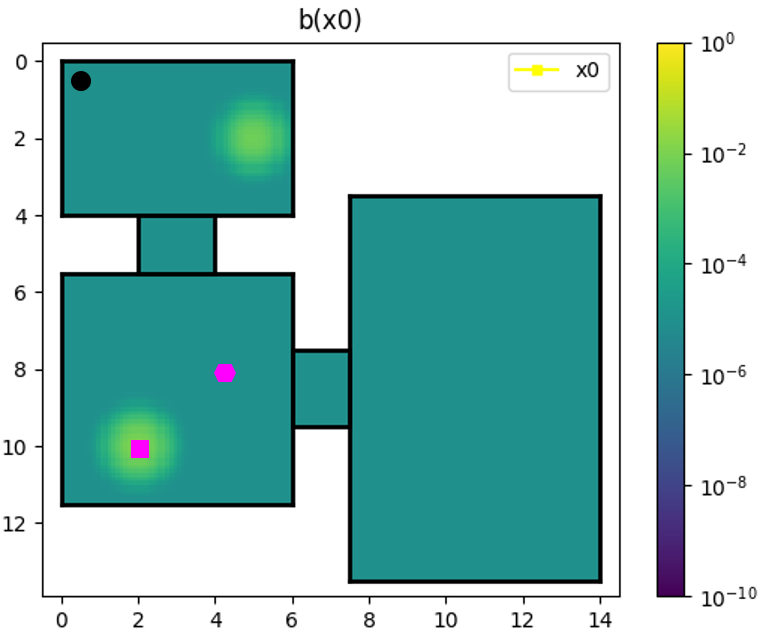
\includegraphics[width=\textwidth]{Report/images/experiments/envsmall_sc01_belief_items.png}
        \caption{Initial configuration}
        \label{subfig:sc01_b0}
    \end{subfigure}
    \hfill
    \begin{subfigure}[b]{0.49\textwidth}
         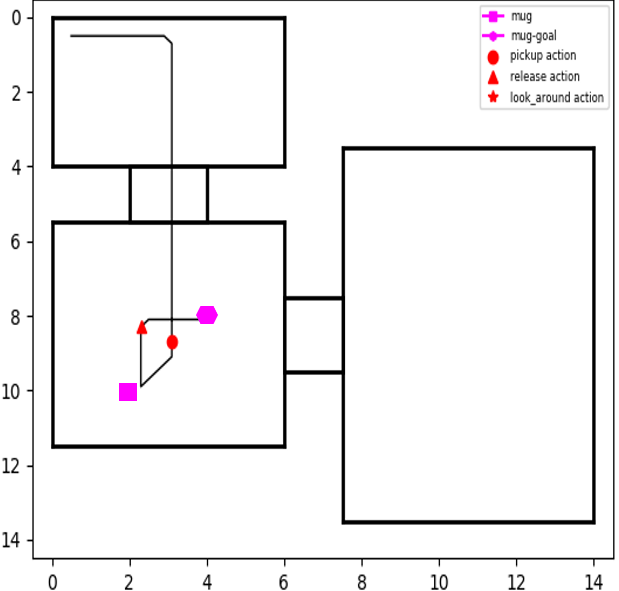
\includegraphics[width=0.82\textwidth]{Report/images/experiments/envsmall_sc01_sol_D1_edited.png}
        \caption{Solution of the Method 01 agent}
        \label{subfig:sc01_sol}
    \end{subfigure}
    \caption{A typical task in the three room environment involving one item. The agent's start position is marked with a black circle, the item's initial position with a pink square and the goal location with a pink hexagon. Image (\subref{subfig:sc01_b0}) shows the initial belief of the item's location and in (\subref{subfig:sc01_sol}) the path of the Method 01 agent is shown. The black line corresponds to the path the agent took, the red circle represents a pickup action and the red triangle a \texttt{release} action.}
    \label{fig:sc01}
\end{figure}

To compare different agents the same scenario is run multiple times where the initial item location is sampled from the initial belief distribution. Figure \ref{subfig:sc01}-\subref{subfig:sc03big} show the initial belief grid of all the scenarios that were tested.
The solution quality is measured as the time the agent took to deliver all items not counting the computation time. Therefore, a small solution quality is preferred. The spread in solution quality within the same agent type is a consequence of sampling the items from the belief distribution. A delivery takes longer if the item is further away from the agent. In Figure \ref{fig:b1vsFlat} the baseline agent, described in Section \ref{sec:baseline}, is compared to the flat POMDP agent from Section \ref{sec:POMDPagent}. The POMDP agent performs better than the baseline agent. The baseline agent does not consider the belief distribution and is not able to reason which item to deliver first, resulting in a longer delivery time (solution quality). For the scenario with broad belief in \ref{subfig:b1vsFlat_sc06} the solution qualities are almost identical, which indicates that the underlying subroutines of the POMDP agent could be improved. For the task in the large environment (see Figure \ref{fig:M1_prob01}) the baseline agent did not find the item in seven of the thirty samples before the simulation was terminated.\\

% %%%%%%%%%%%%%%%%%%%%%%%%%%%%%%%%%%%%%%%%%%%%%%%%%%%%%%%%%%%%%%%%%%%%%%%%%%%%%%%%%%%%%
% %%%%%%%%%%%%%%%%%%%%%%%%%%%%%%%%%%%%%%%%%%%%%%%%%%%%%%%%%%%%%%%%%%%%%%%%%%%%%%%%%%%%%
\begin{figure}
    \centering
    \begin{subfigure}[t]{0.49\textwidth}
        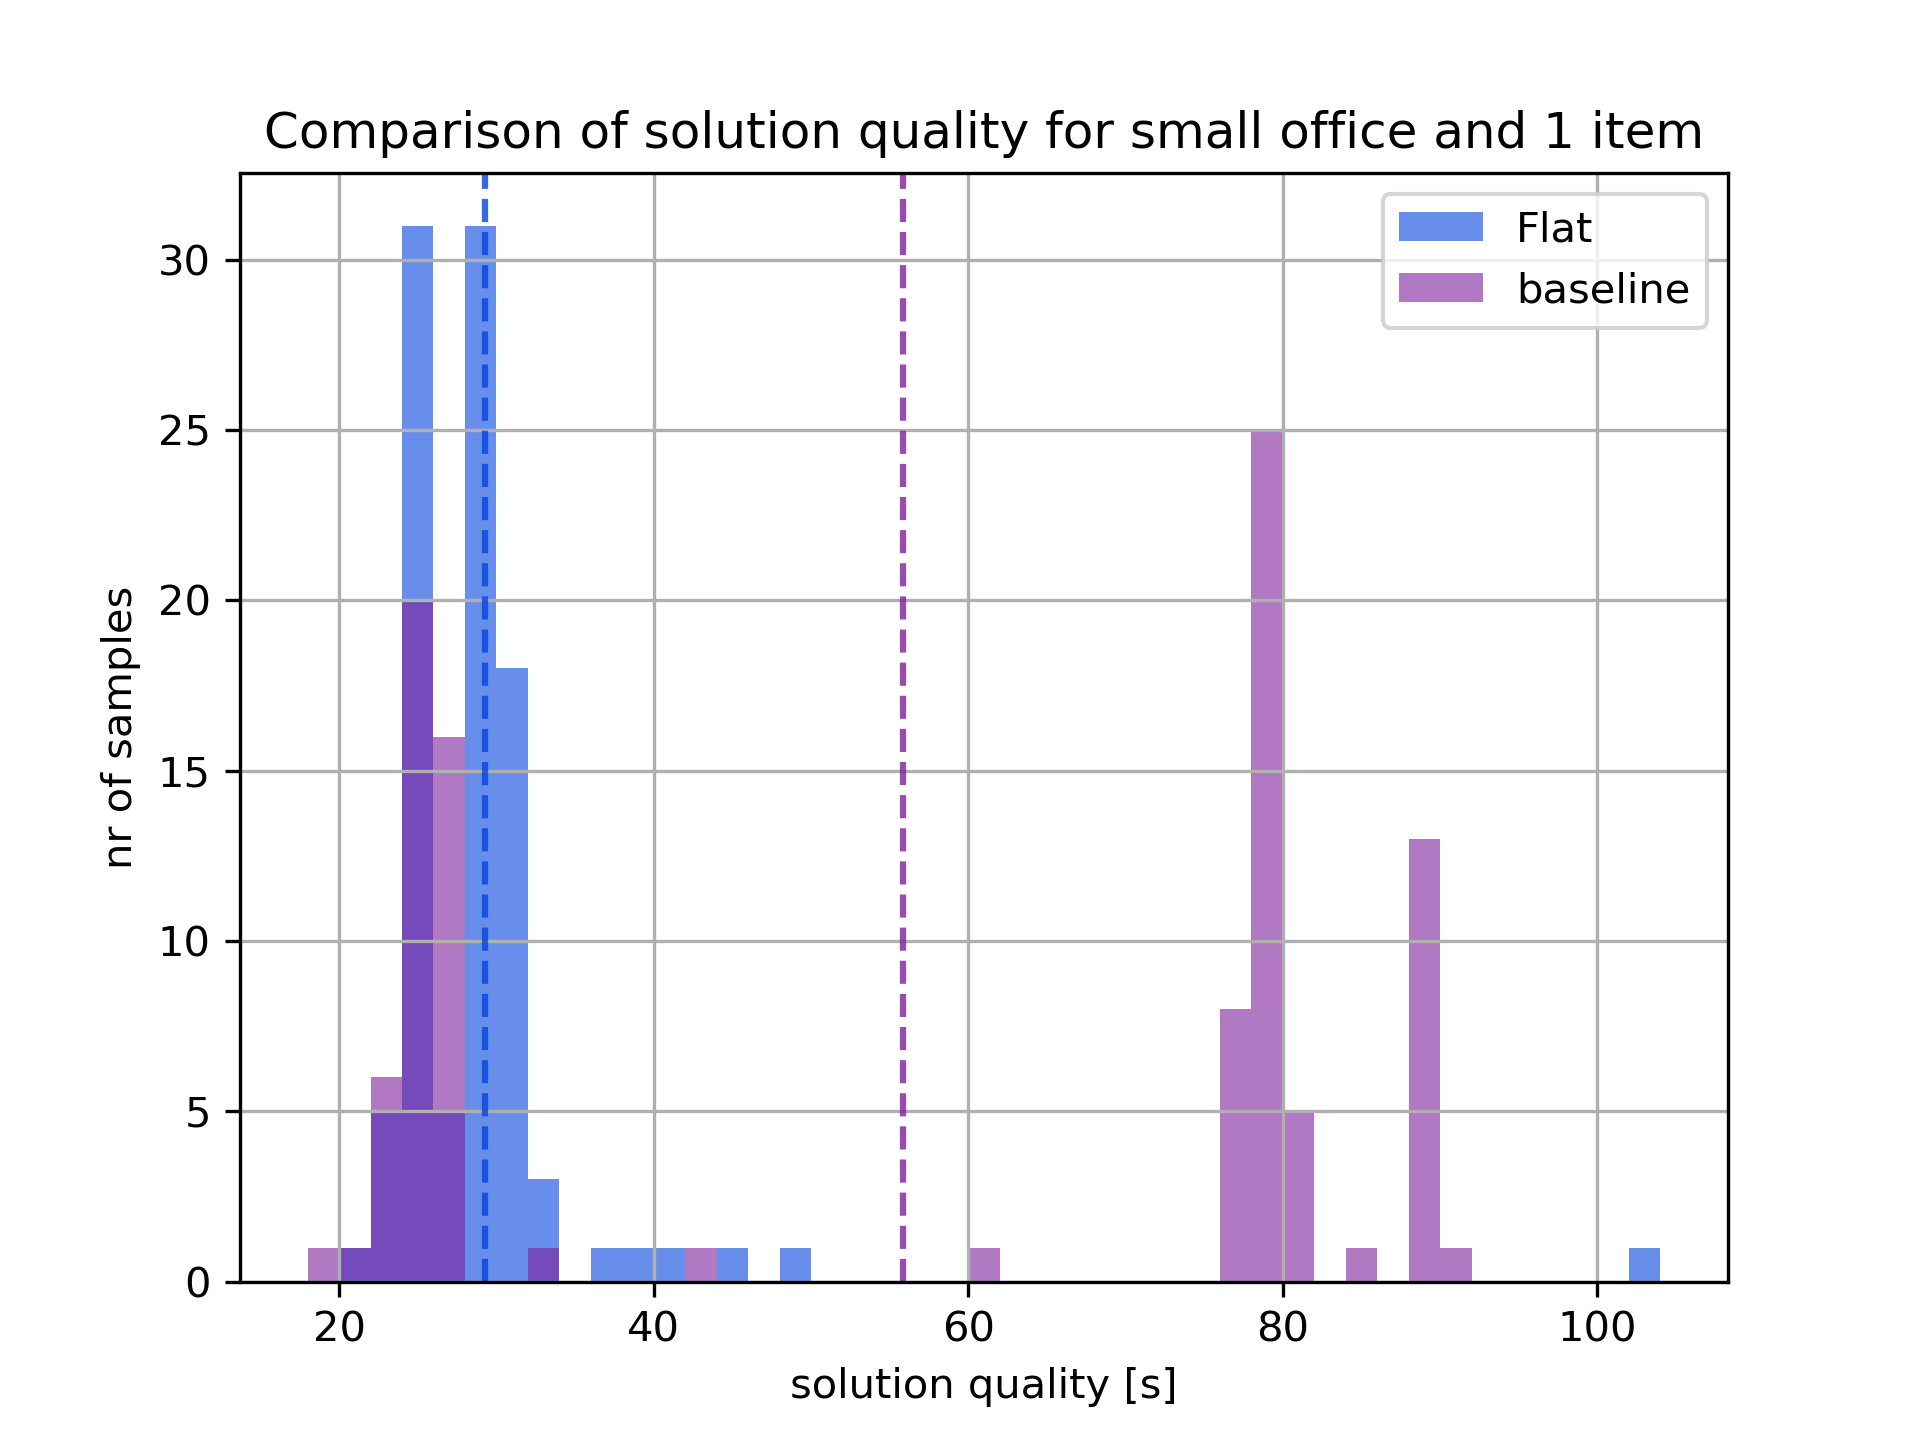
\includegraphics[width=\textwidth]{Report/images/sol_quality/envsmall_sc01_solqual_hist.png}
        \caption{Scenario from Figure \ref{fig:sc01}}
        \label{subfig:b1vsFlat_sc01}
    \end{subfigure}
    \begin{subfigure}[t]{0.49\textwidth}
         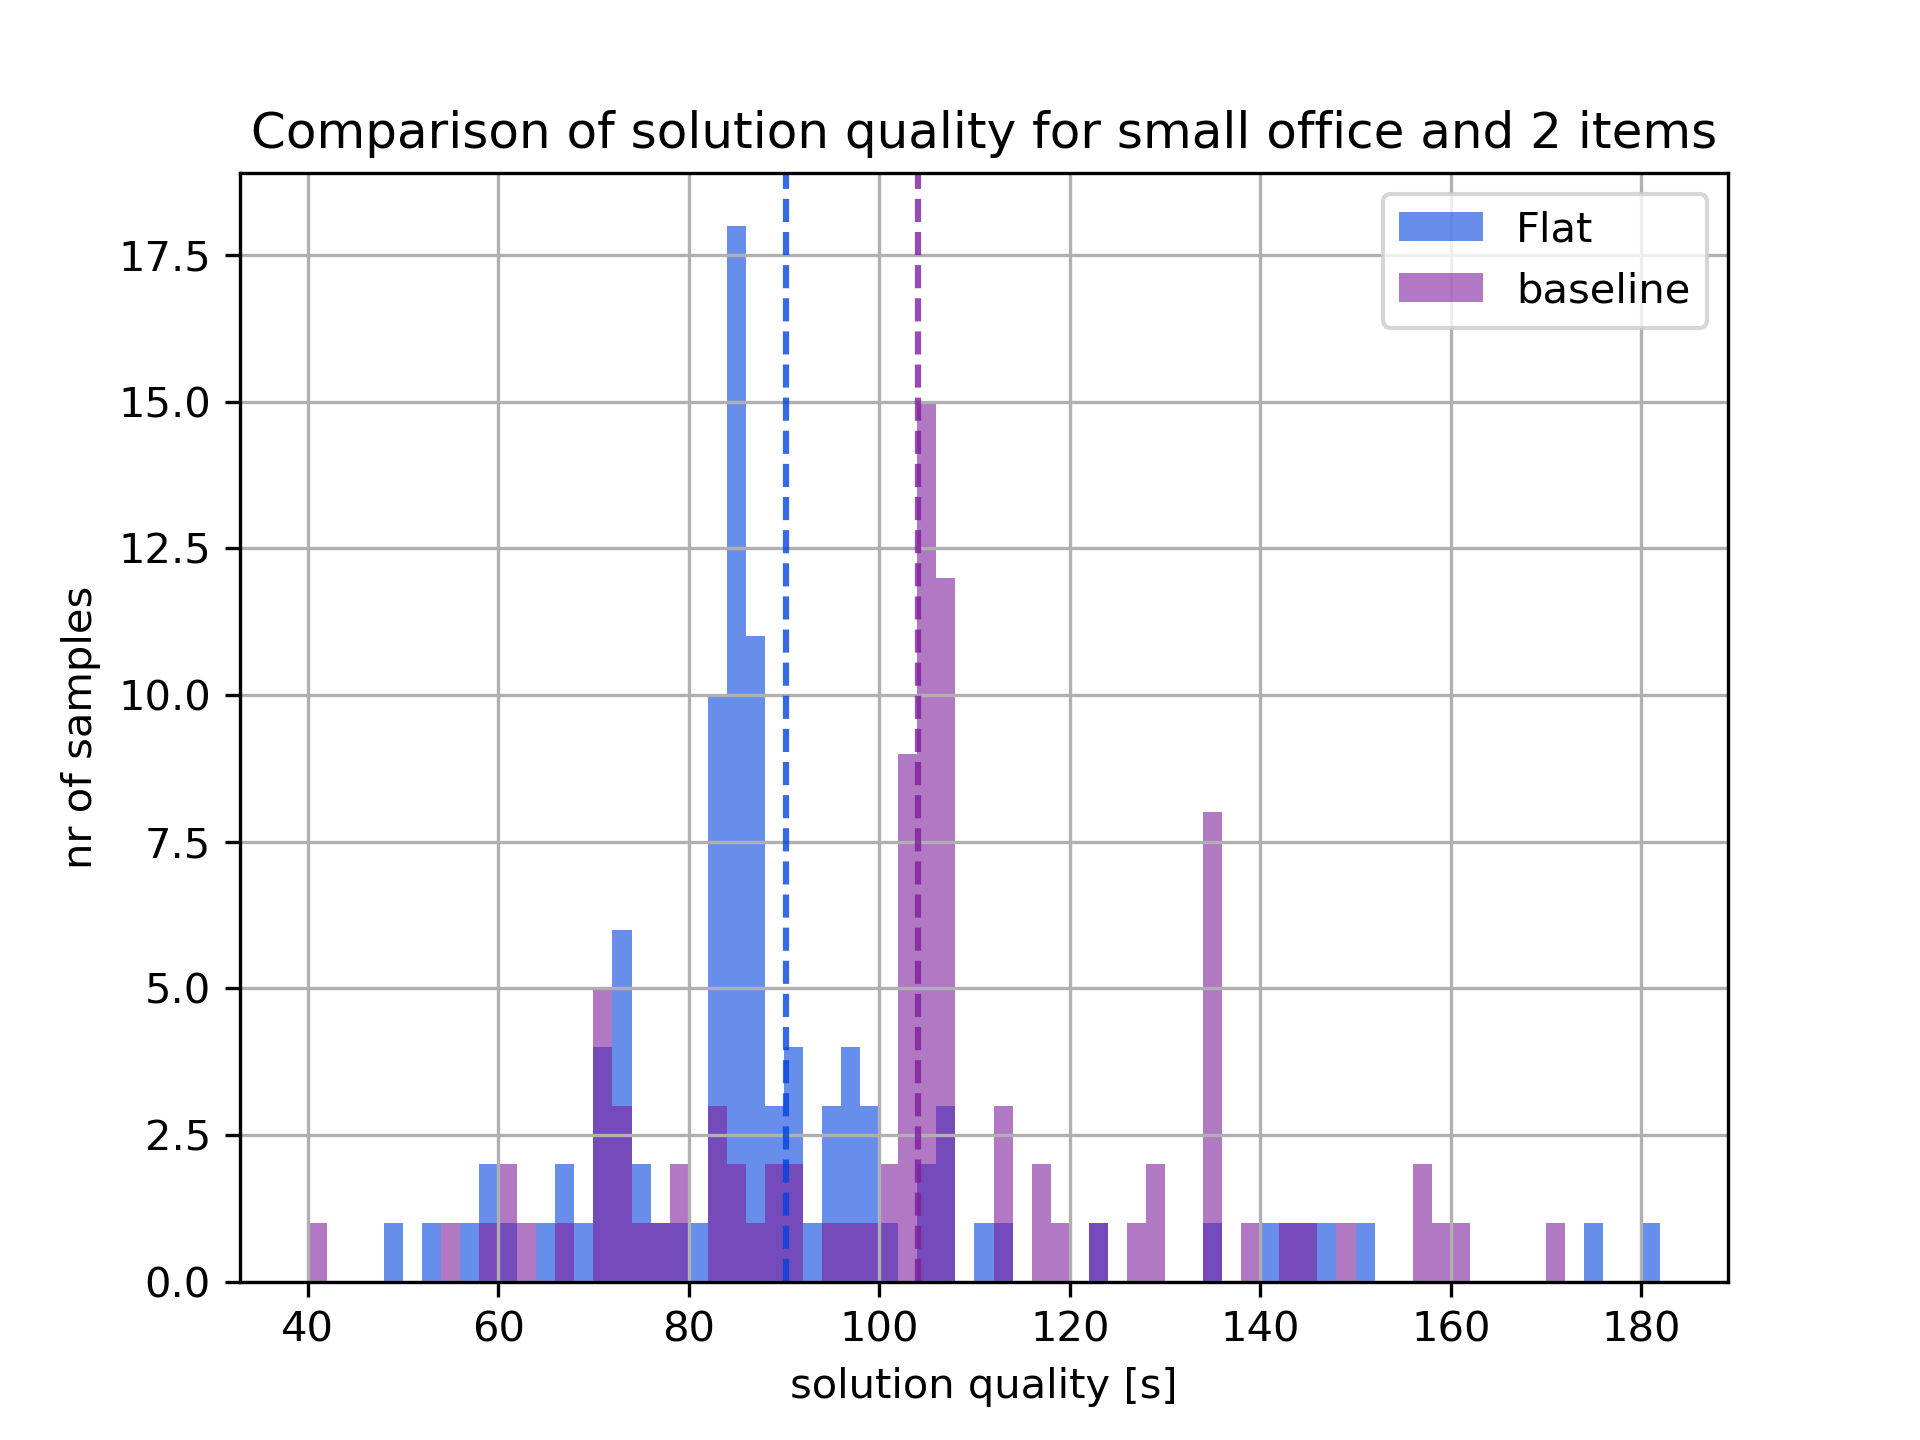
\includegraphics[width=\textwidth]{Report/images/sol_quality/envsmall_sc04_solqual_hist.png}
        \caption{Two items task with few belief peaks, scenario shown in Figure \ref{subfig:sc04}}
        \label{subfig:b1vsFlat_sc04}
    \end{subfigure}
    \hfill
    \begin{subfigure}[t]{0.49\textwidth}
        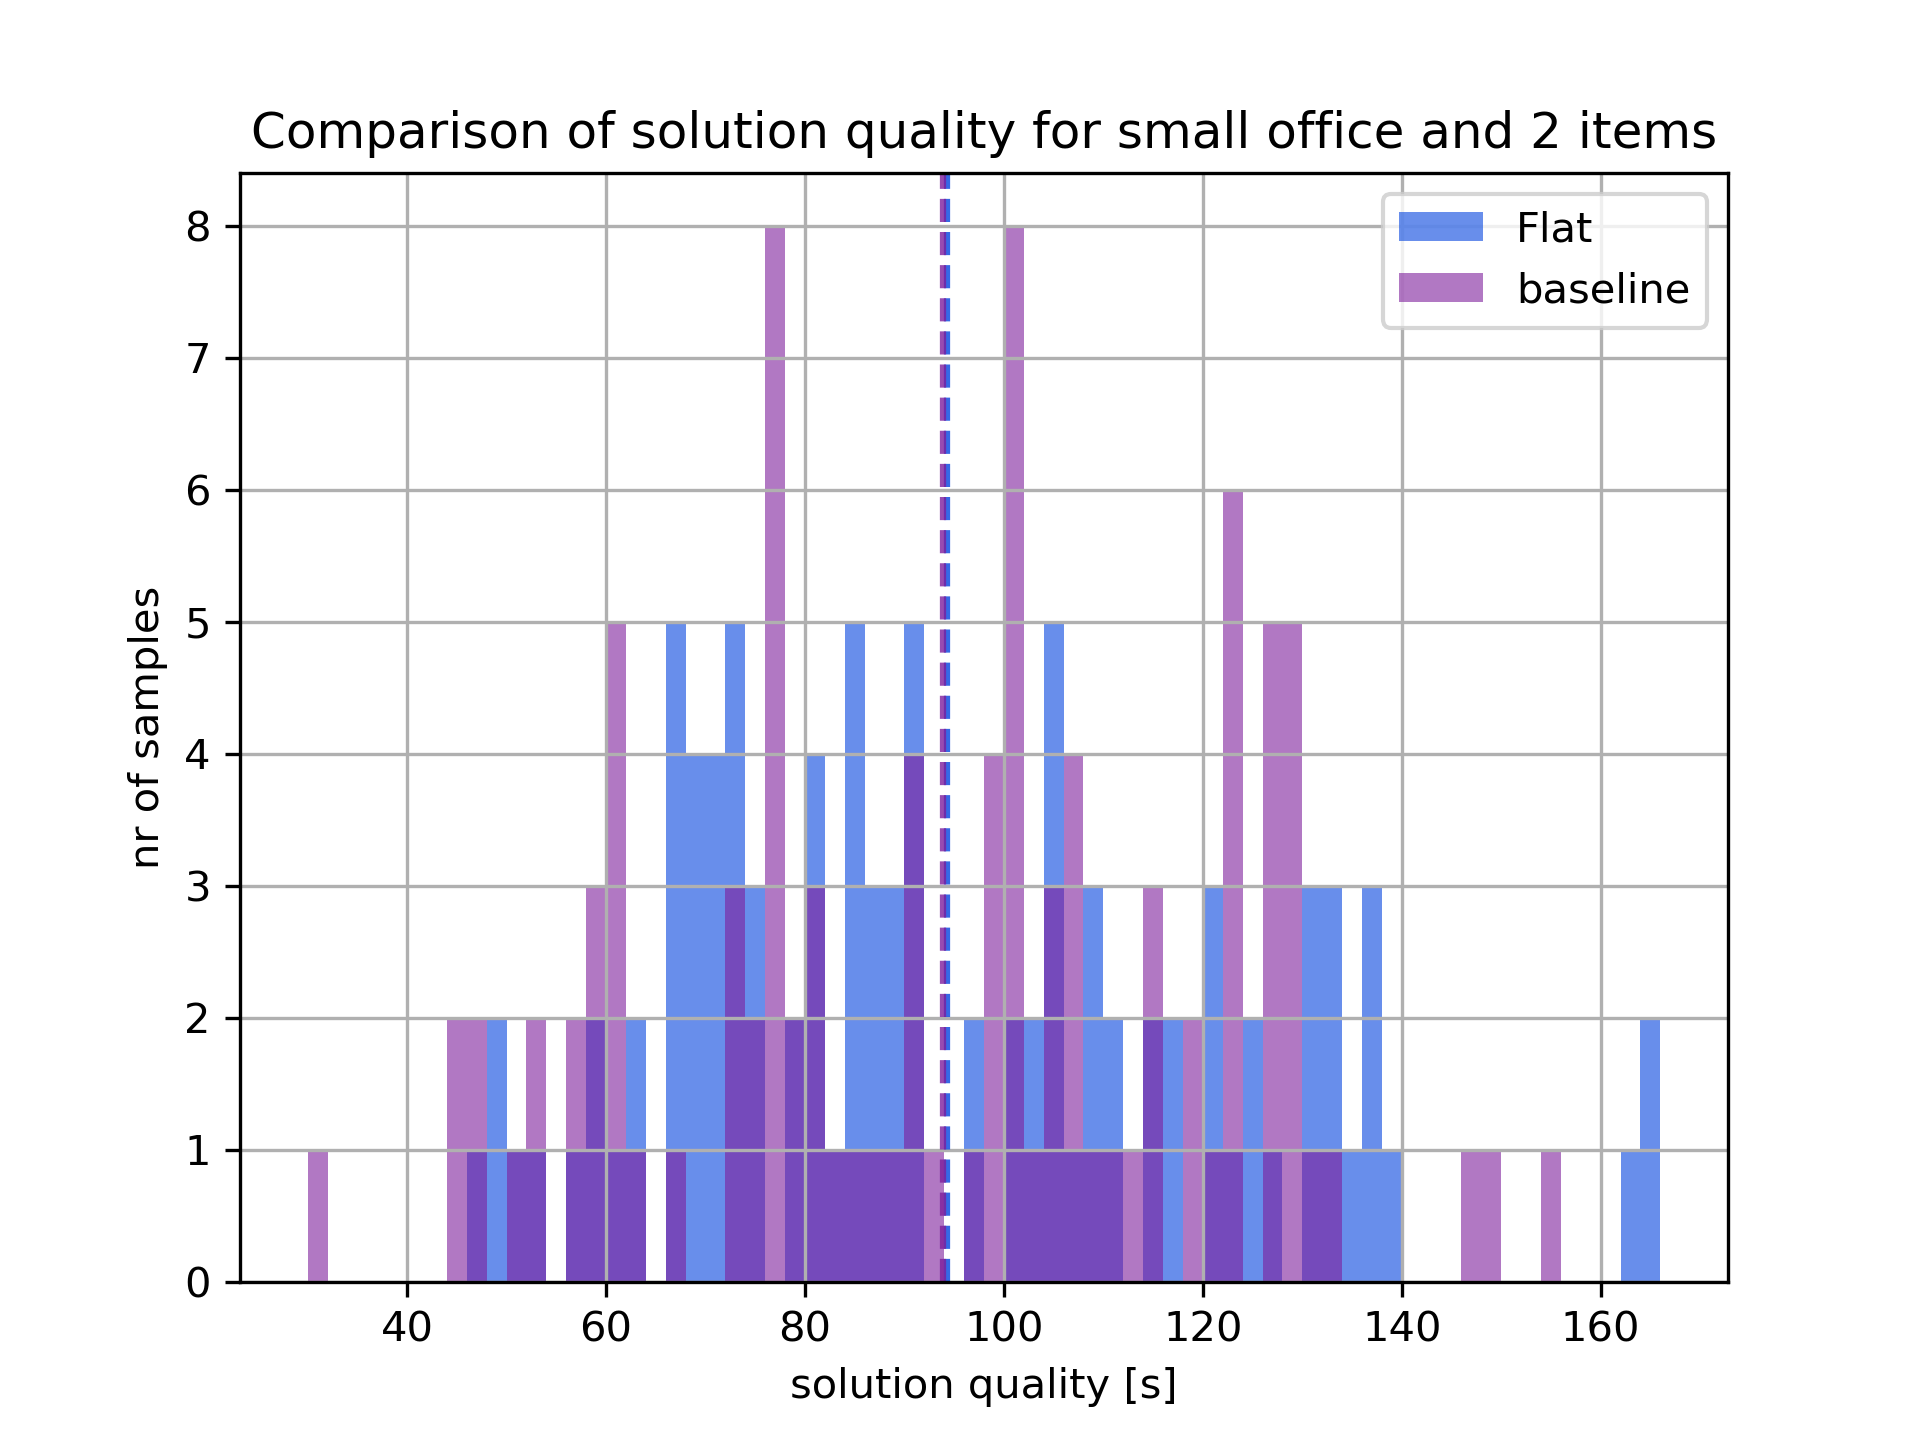
\includegraphics[width=\textwidth]{Report/images/sol_quality/envsmall_sc06_solqual_hist.png}
        \caption{Two items task with broad belief distribution, scenario shown in Figure \ref{subfig:sc06}}
        \label{subfig:b1vsFlat_sc06}
    \end{subfigure}
    \hfill
    \begin{subfigure}[t]{0.49\textwidth}
         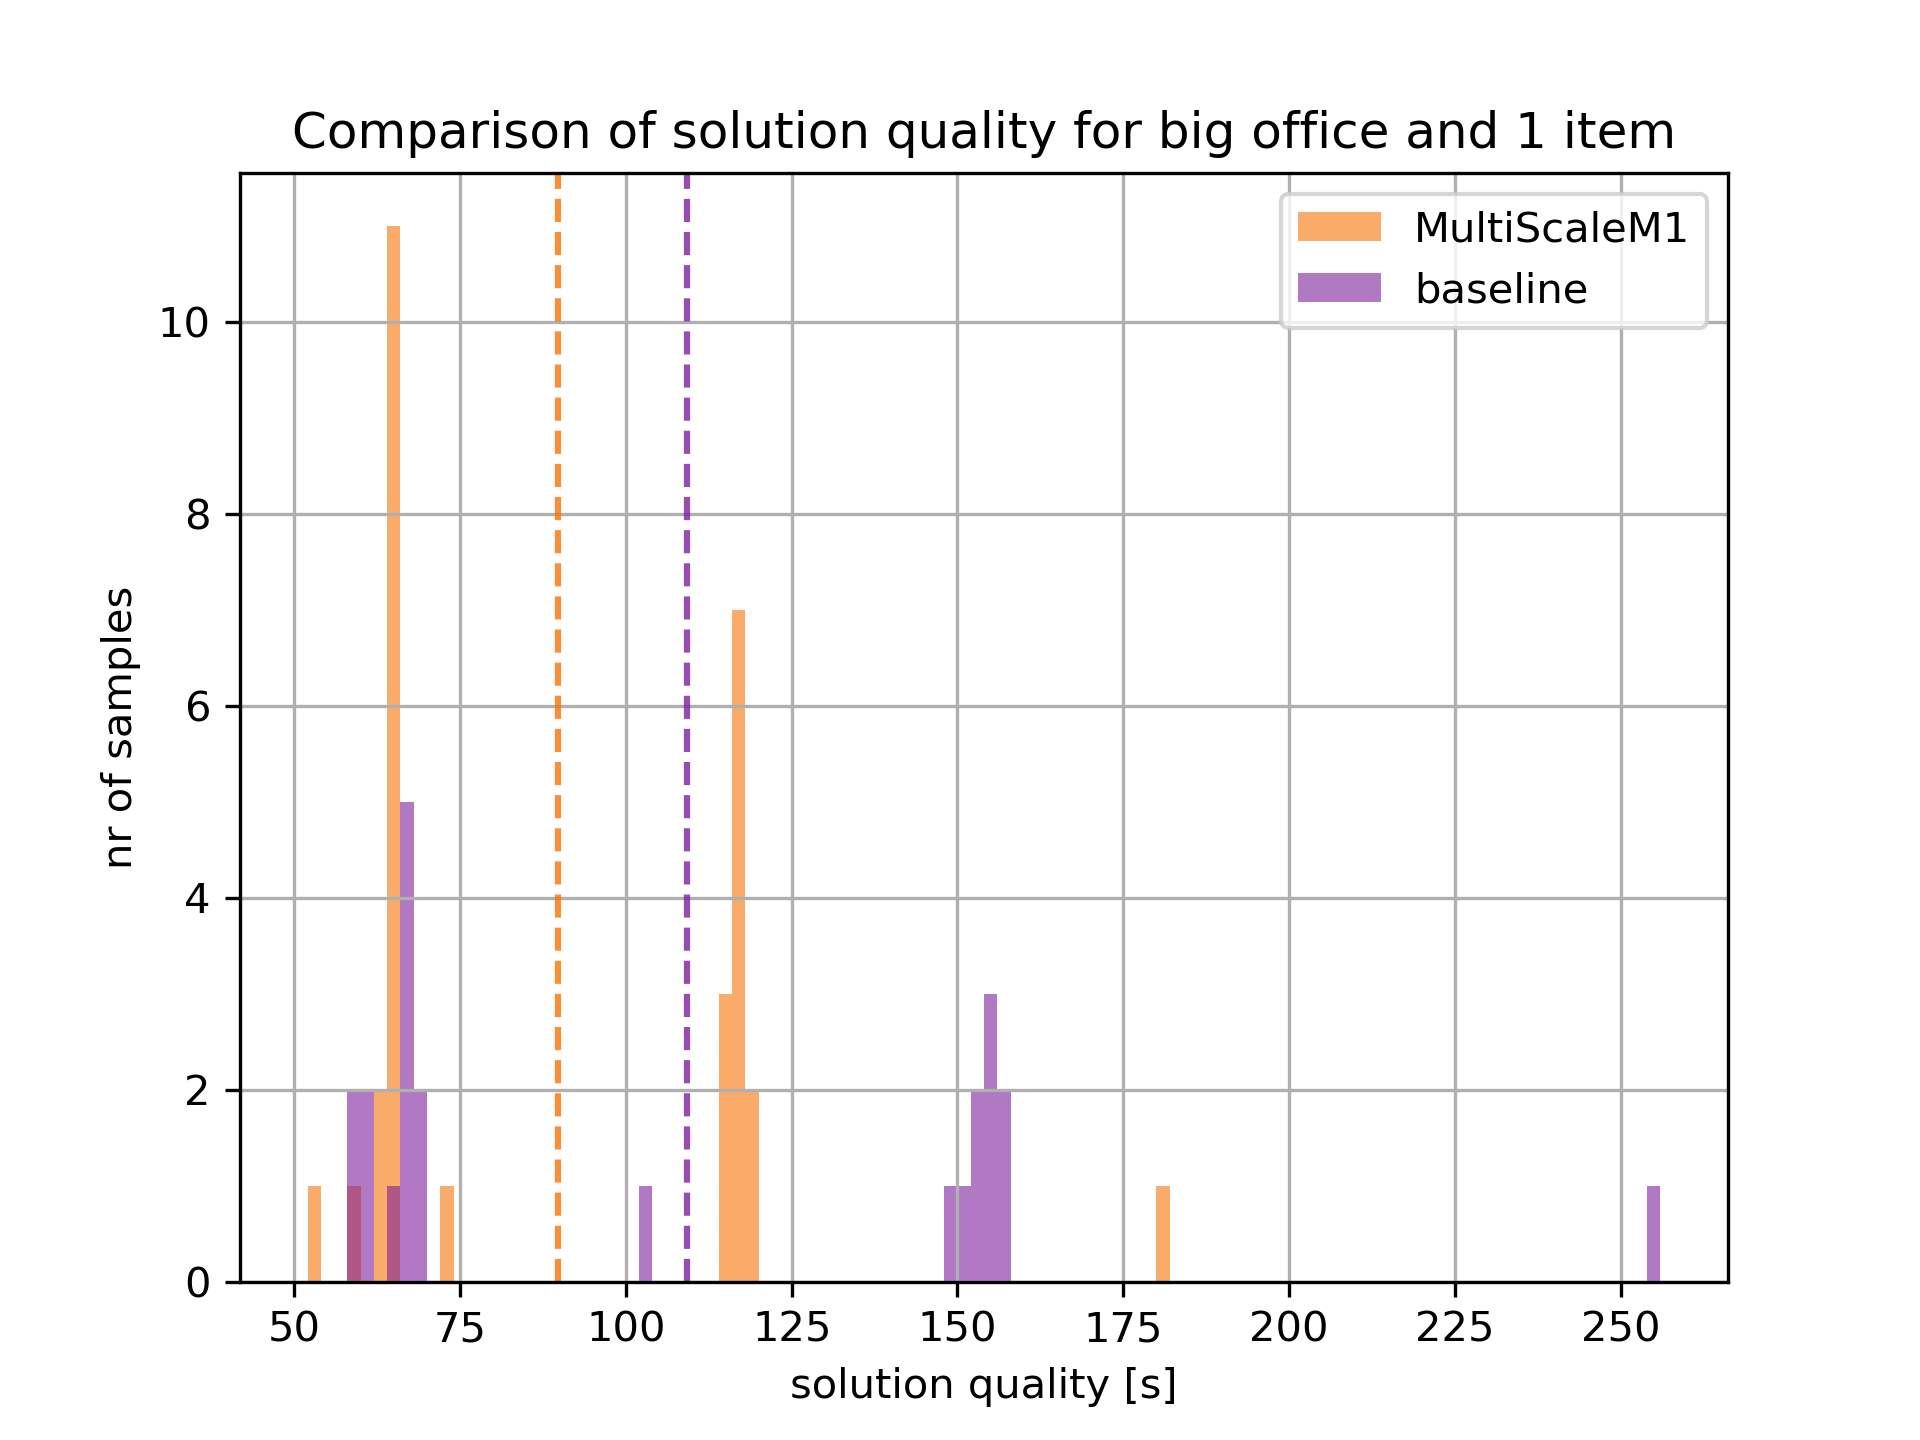
\includegraphics[width=\textwidth]{Report/images/sol_quality/envbig_sc01_solqual_hist.png}
        \caption{One item task in large environment, scenario shown in Figure \ref{subfig:sc01big} }
        \label{subfig:b1vsFlat_sc01Big}
    \end{subfigure}
    \caption{Comparison in solution quality between the baseline agent and the POMDP agents. In (\subref{subfig:b1vsFlat_sc01}), (\subref{subfig:b1vsFlat_sc04}) and (\subref{subfig:b1vsFlat_sc06}) 100 samples are used. In (\subref{subfig:b1vsFlat_sc01Big}) 30 samples are used but 7 were removed for the baseline agent as it was not able to find the item before the termination time of the simulation was reached. In (\subref{subfig:b1vsFlat_sc01}), (\subref{subfig:b1vsFlat_sc04}) and (\subref{subfig:b1vsFlat_sc06}) the flat POMDP agent is shown and in (\subref{subfig:b1vsFlat_sc01Big}) the Multi-Scale Method 01.}
    \label{fig:b1vsFlat}
\end{figure}
% %%%%%%%%%%%%%%%%%%%%%%%%%%%%%%%%%%%%%%%%%%%%%%%%%%%%%%%%%%%%%%%%%%%%%%%%%%%%%%%%%
% %%%%%%%%%%%%%%%%%%%%%%%%%%%%%%%%%%%%%%%%%%%%%%%%%%%%%%%%%%%%%%%%%%%%%%%%%%%%%%%%%
\begin{figure}
    \centering
    \begin{subfigure}[b]{0.49\textwidth}
        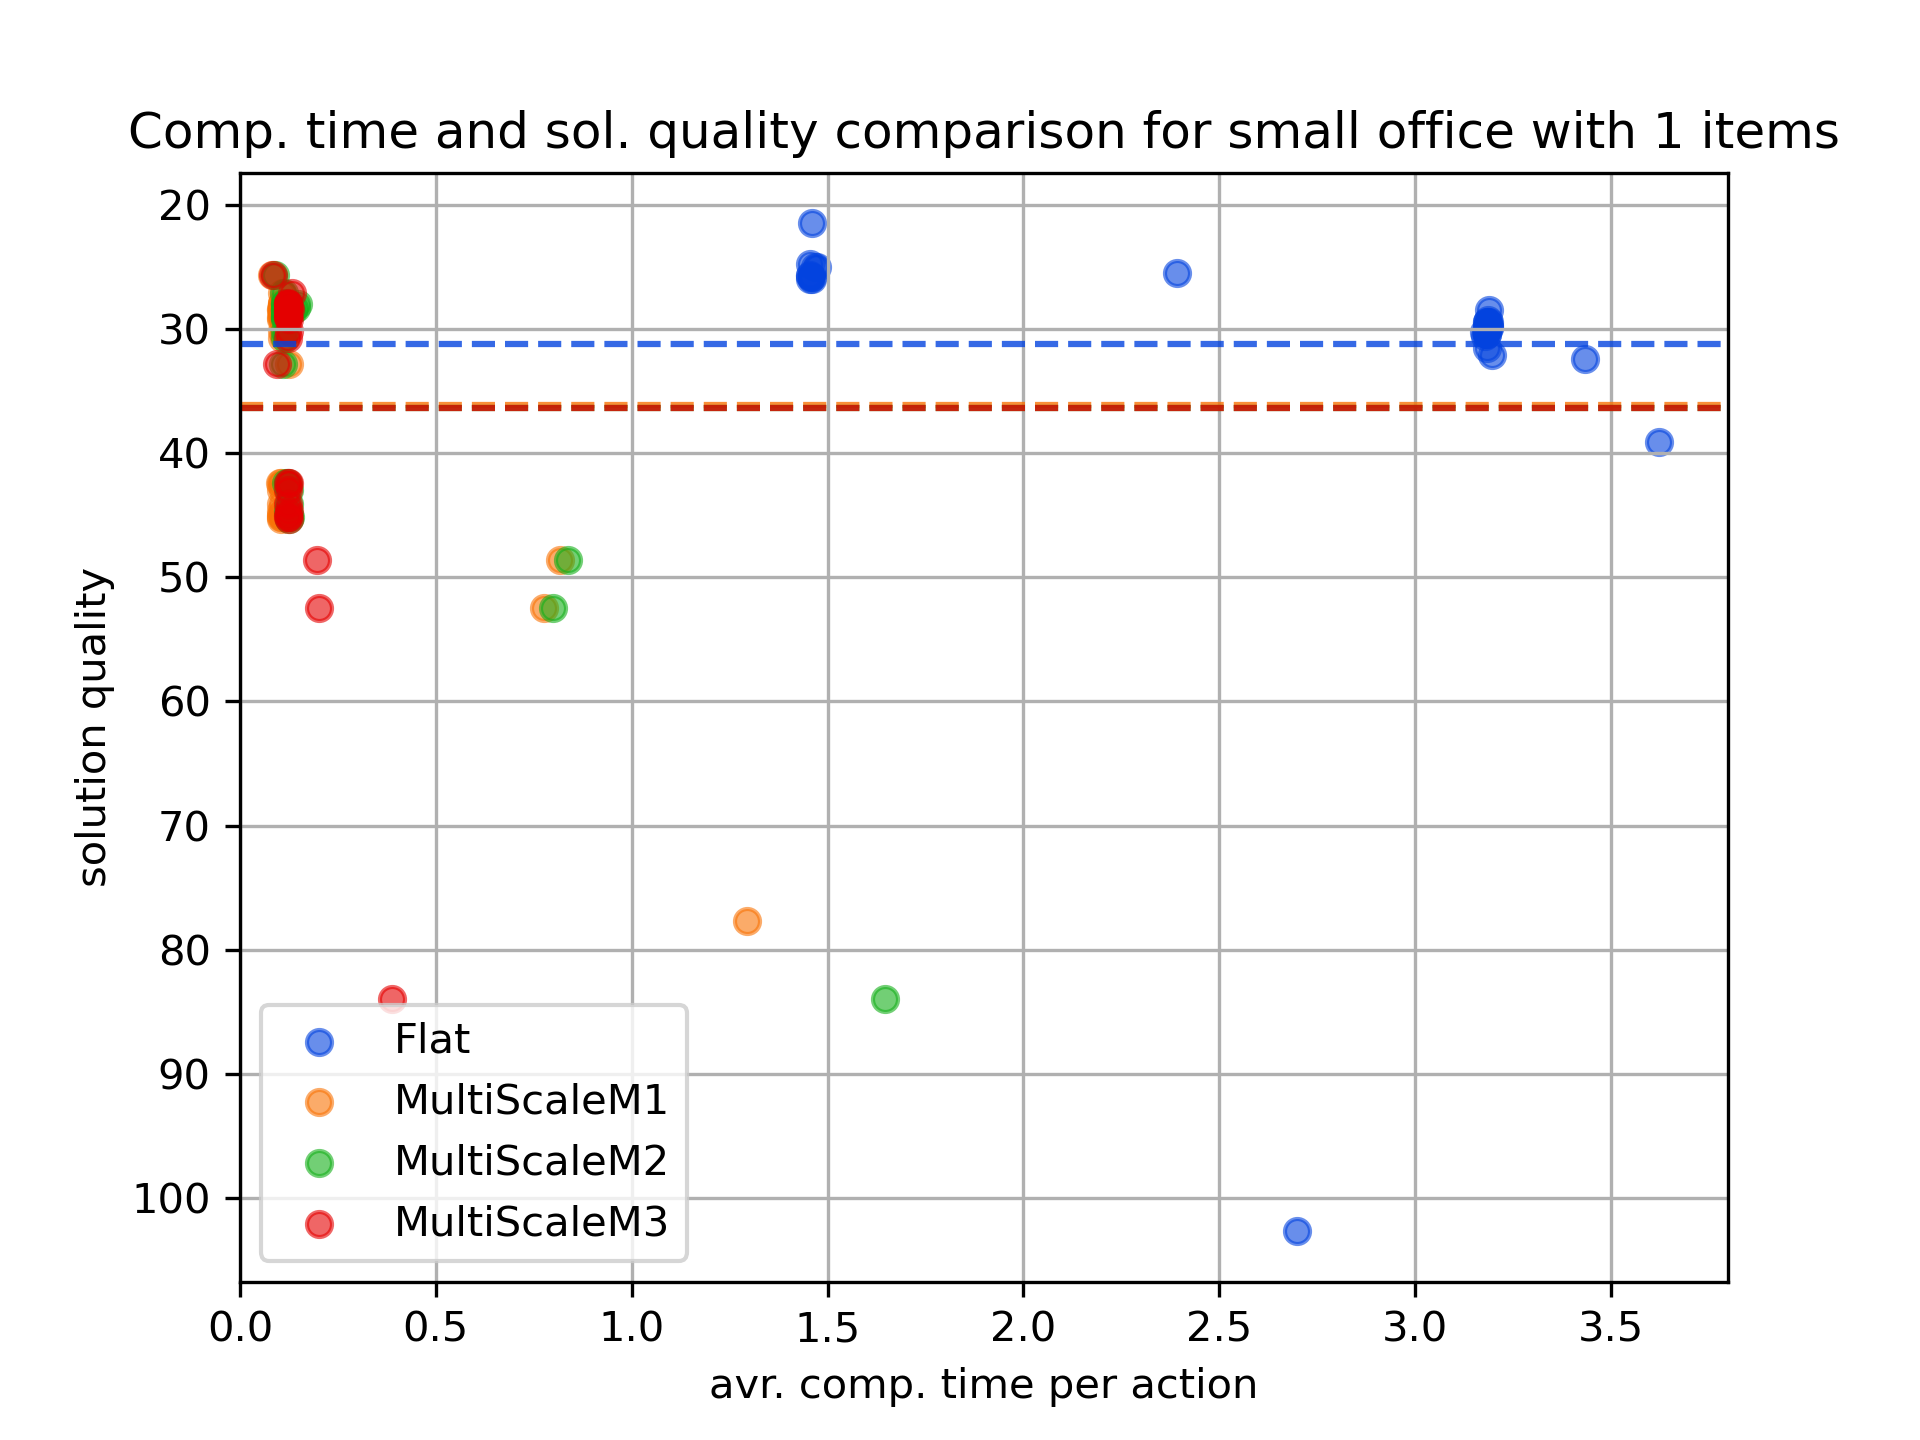
\includegraphics[width=\textwidth]{Report/images/comp_time_vs_sol_quality/envsmall_sc01_scatter_comptimes_vs_solqual.png}
        \caption{Scenario from figure \ref{fig:sc01}}
        \label{subfig:comp_sc01}
    \end{subfigure}
    \begin{subfigure}[b]{0.49\textwidth}
         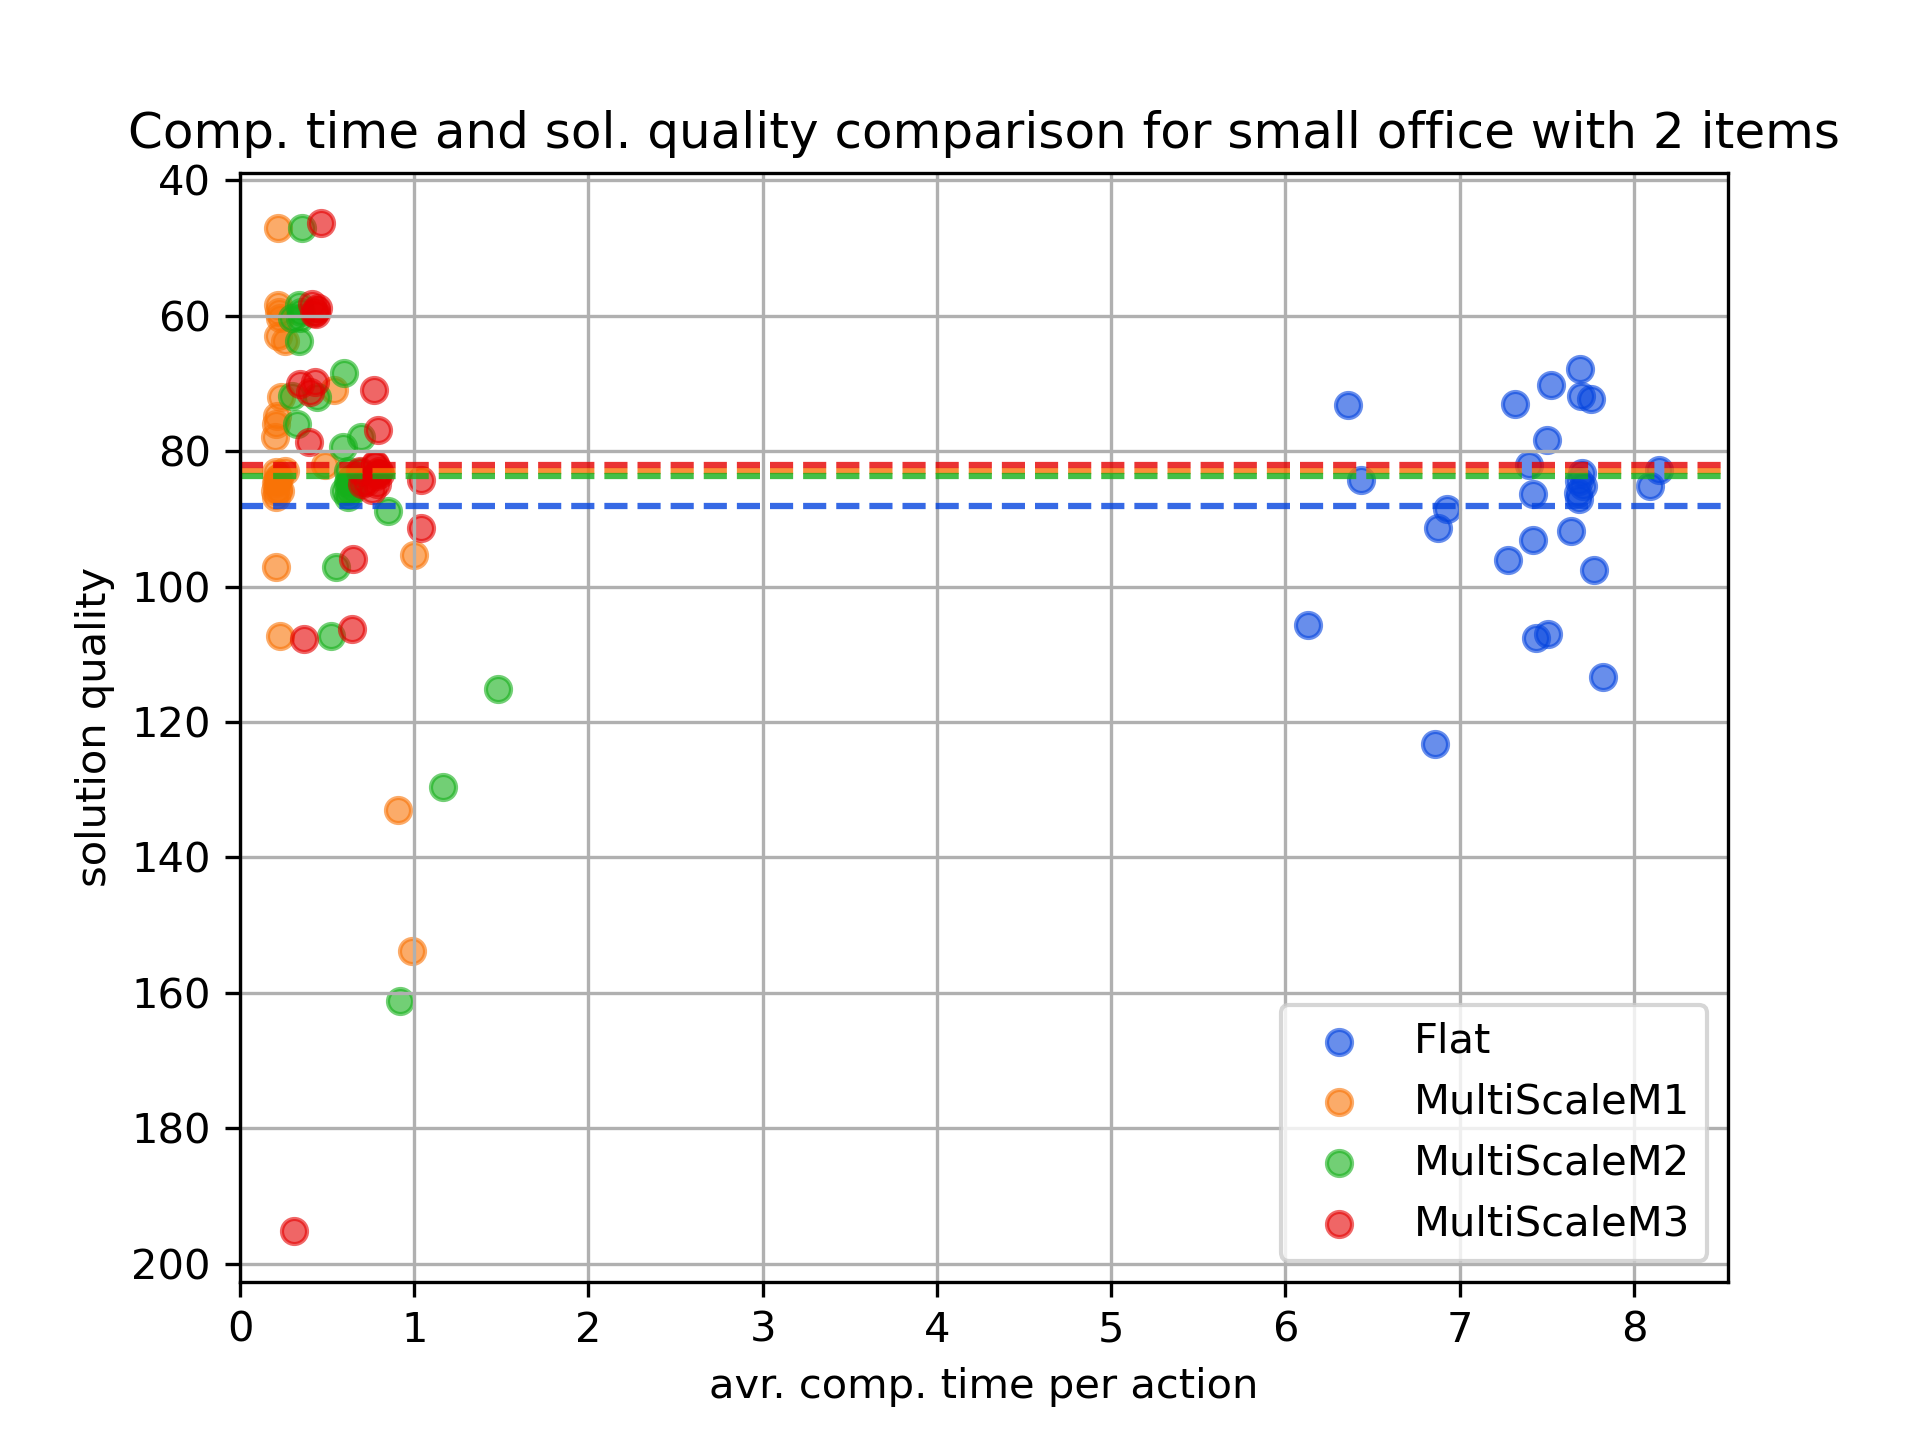
\includegraphics[width=\textwidth]{Report/images/comp_time_vs_sol_quality/envsmall_sc04_scatter_comptimes_vs_solqual.png}
        \caption{Two items scenario with few belief peaks, scenario shown in Figure \ref{subfig:sc04}}
        \label{subfig:comp_sc04}
    \end{subfigure}
    \hfill
    \begin{subfigure}[b]{0.49\textwidth}
        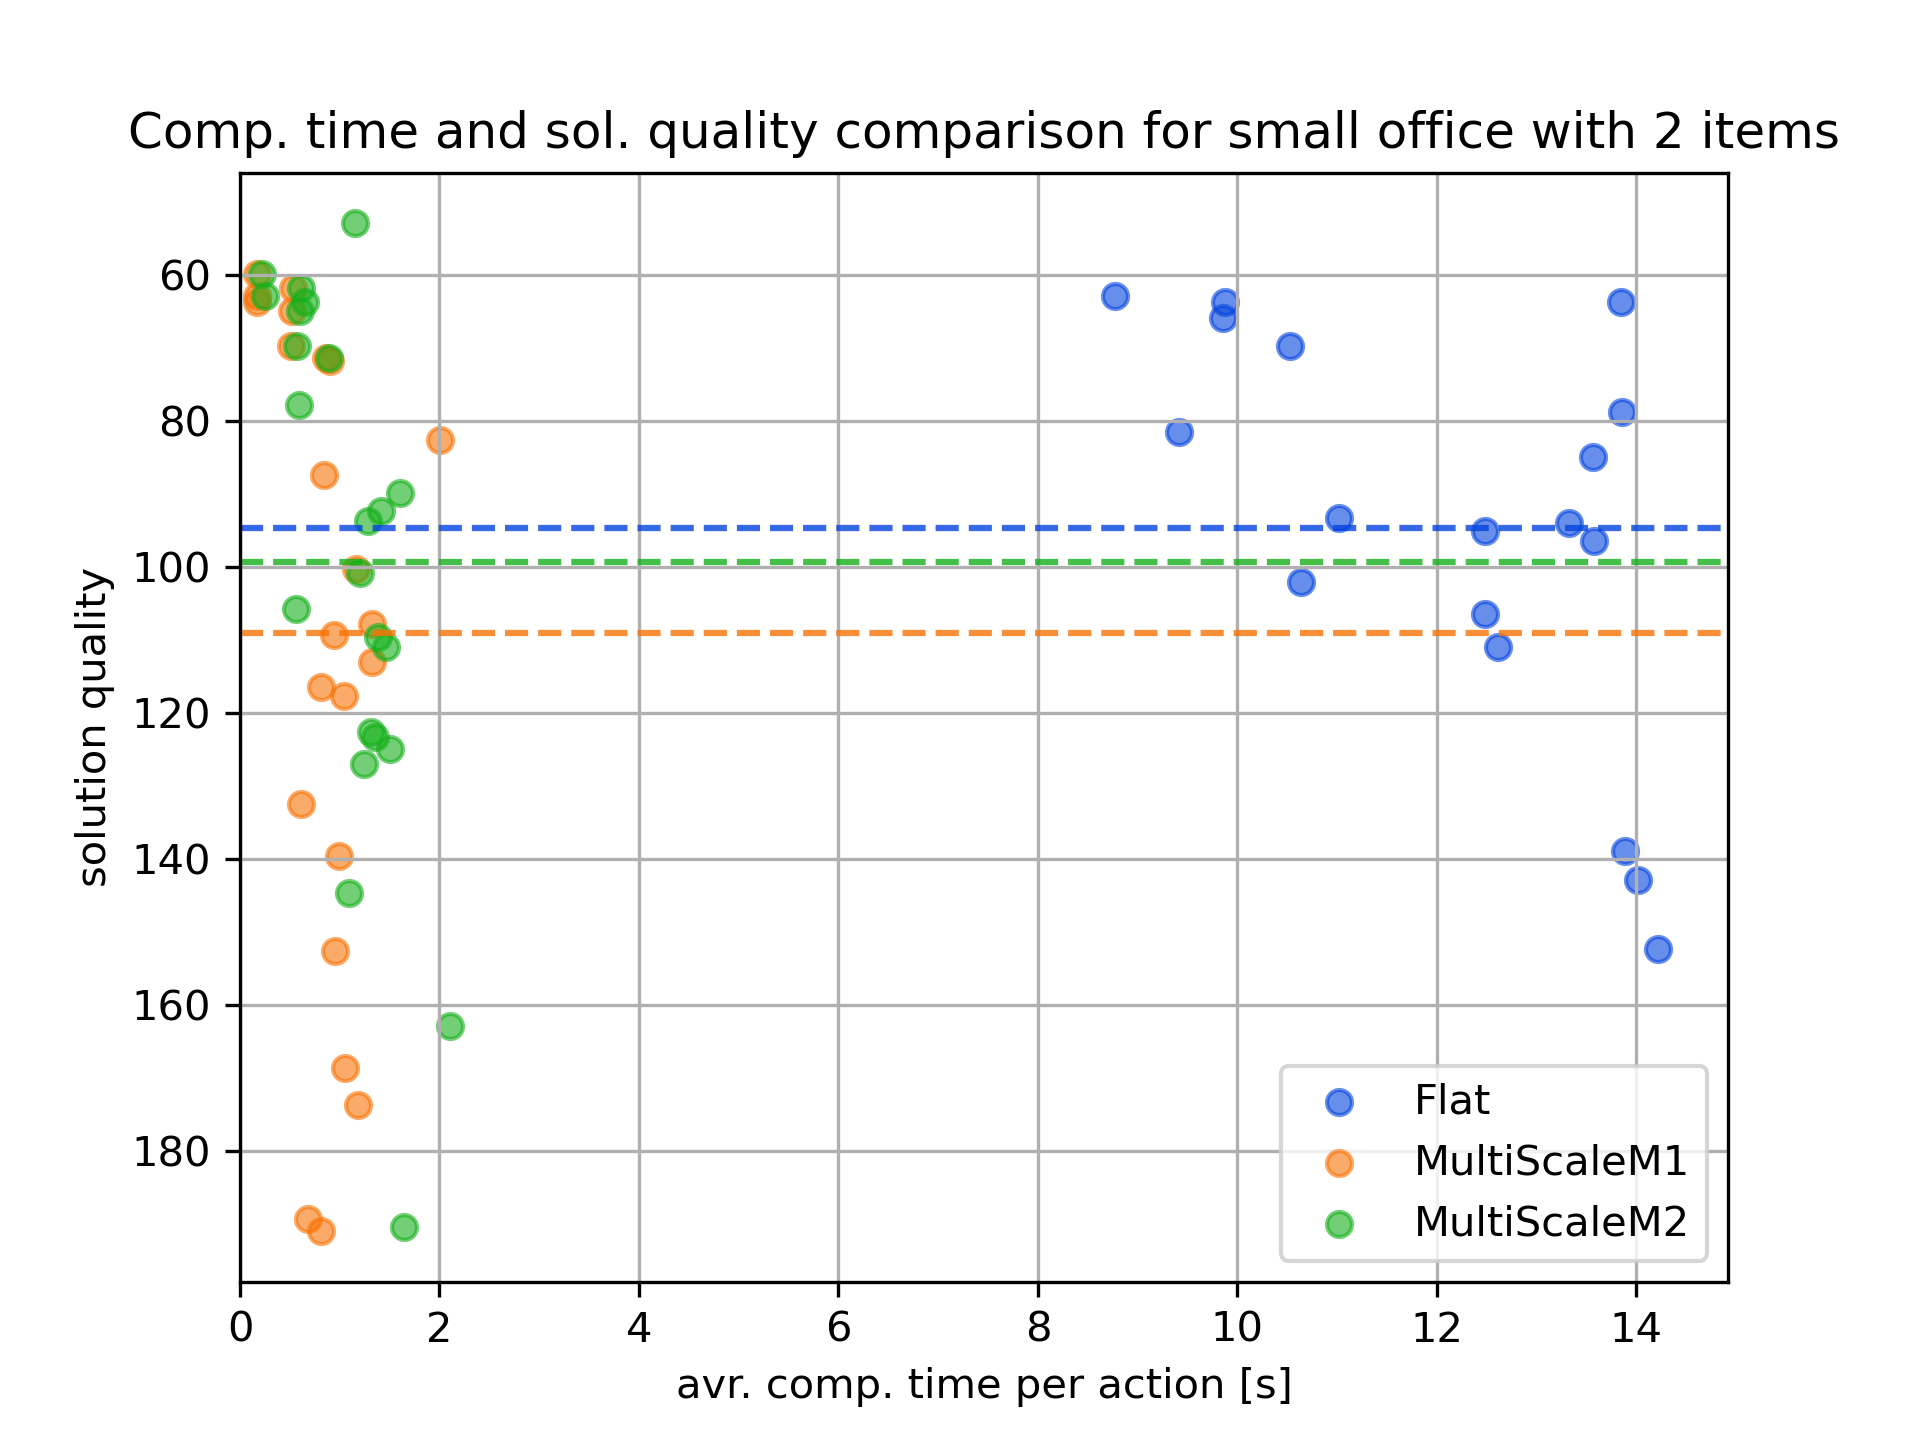
\includegraphics[width=\textwidth]{Report/images/comp_time_vs_sol_quality/envsmall_sc08_scatter_comptimes_vs_solqual.png}
        \caption{Two items task with uniform initial belief, scenario shown in Figure \ref{subfig:sc08}}
        \label{subfig:comp_sc08}
    \end{subfigure}
    \hfill
    \begin{subfigure}[b]{0.49\textwidth}
         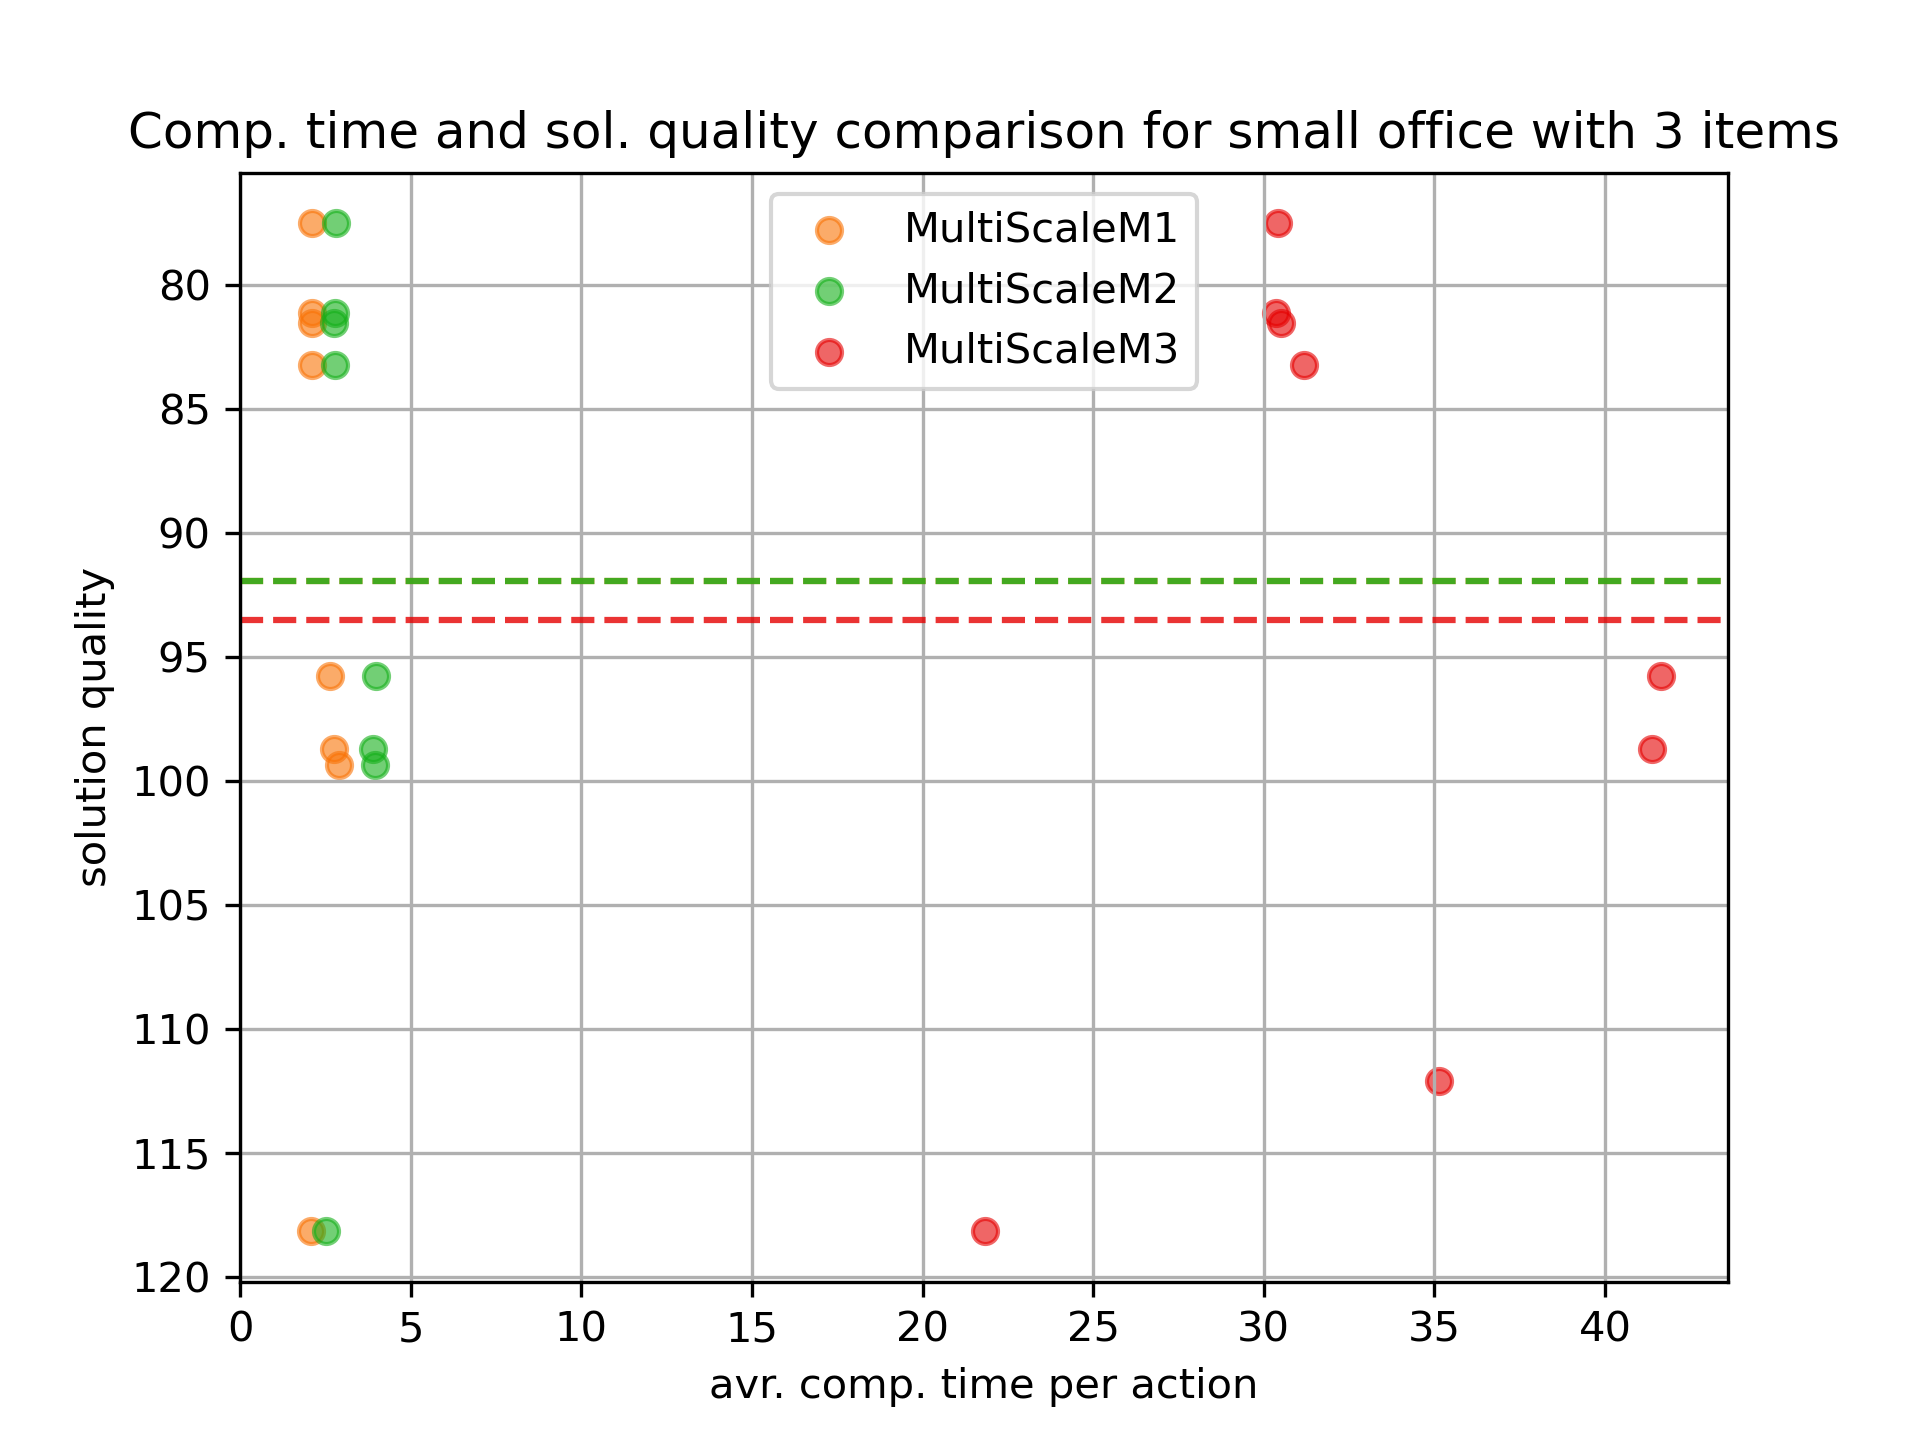
\includegraphics[width=\textwidth]{Report/images/comp_time_vs_sol_quality/envsmall_sc09_scatter_comptimes_vs_solqual.png}
        \caption{Three items task with few belief peaks, scenario shown in Figure \ref{subfig:sc09}}
        \label{subfig:comp_sc09}
    \end{subfigure}
        \hfill
    \begin{subfigure}[b]{0.49\textwidth}
        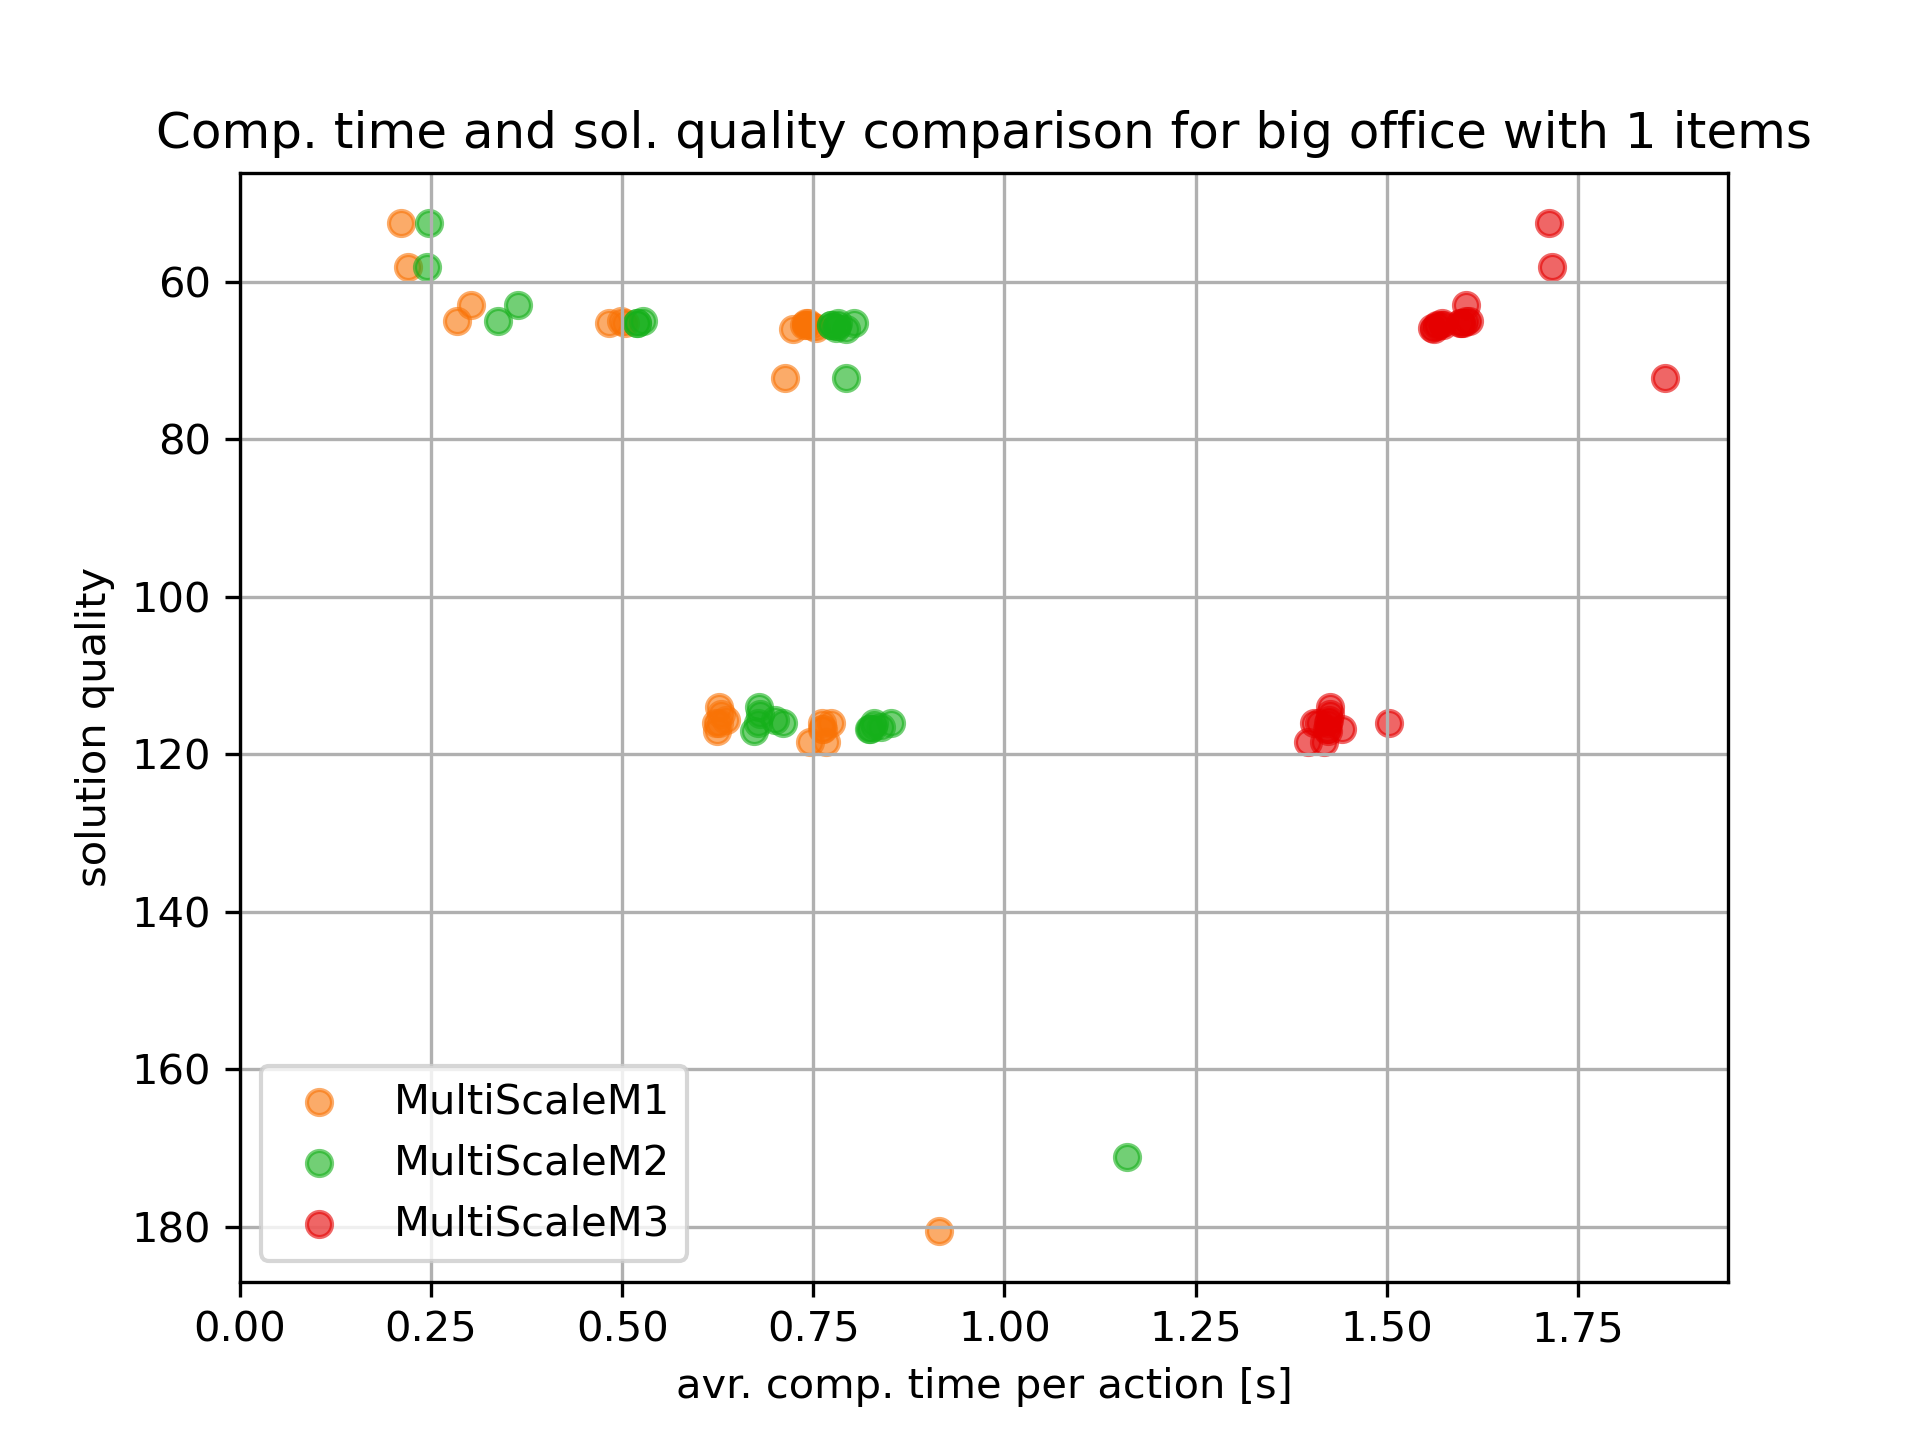
\includegraphics[width=\textwidth]{Report/images/comp_time_vs_sol_quality/envbig_sc01_noavr_scatter_comptimes_vs_solqual.png}
        \caption{One item task in large environment, scenario shown in Figure \ref{subfig:sc01big}}
        \label{subfig:comp_sc01Big}
    \end{subfigure}
    \hfill
    \begin{subfigure}[b]{0.49\textwidth}
         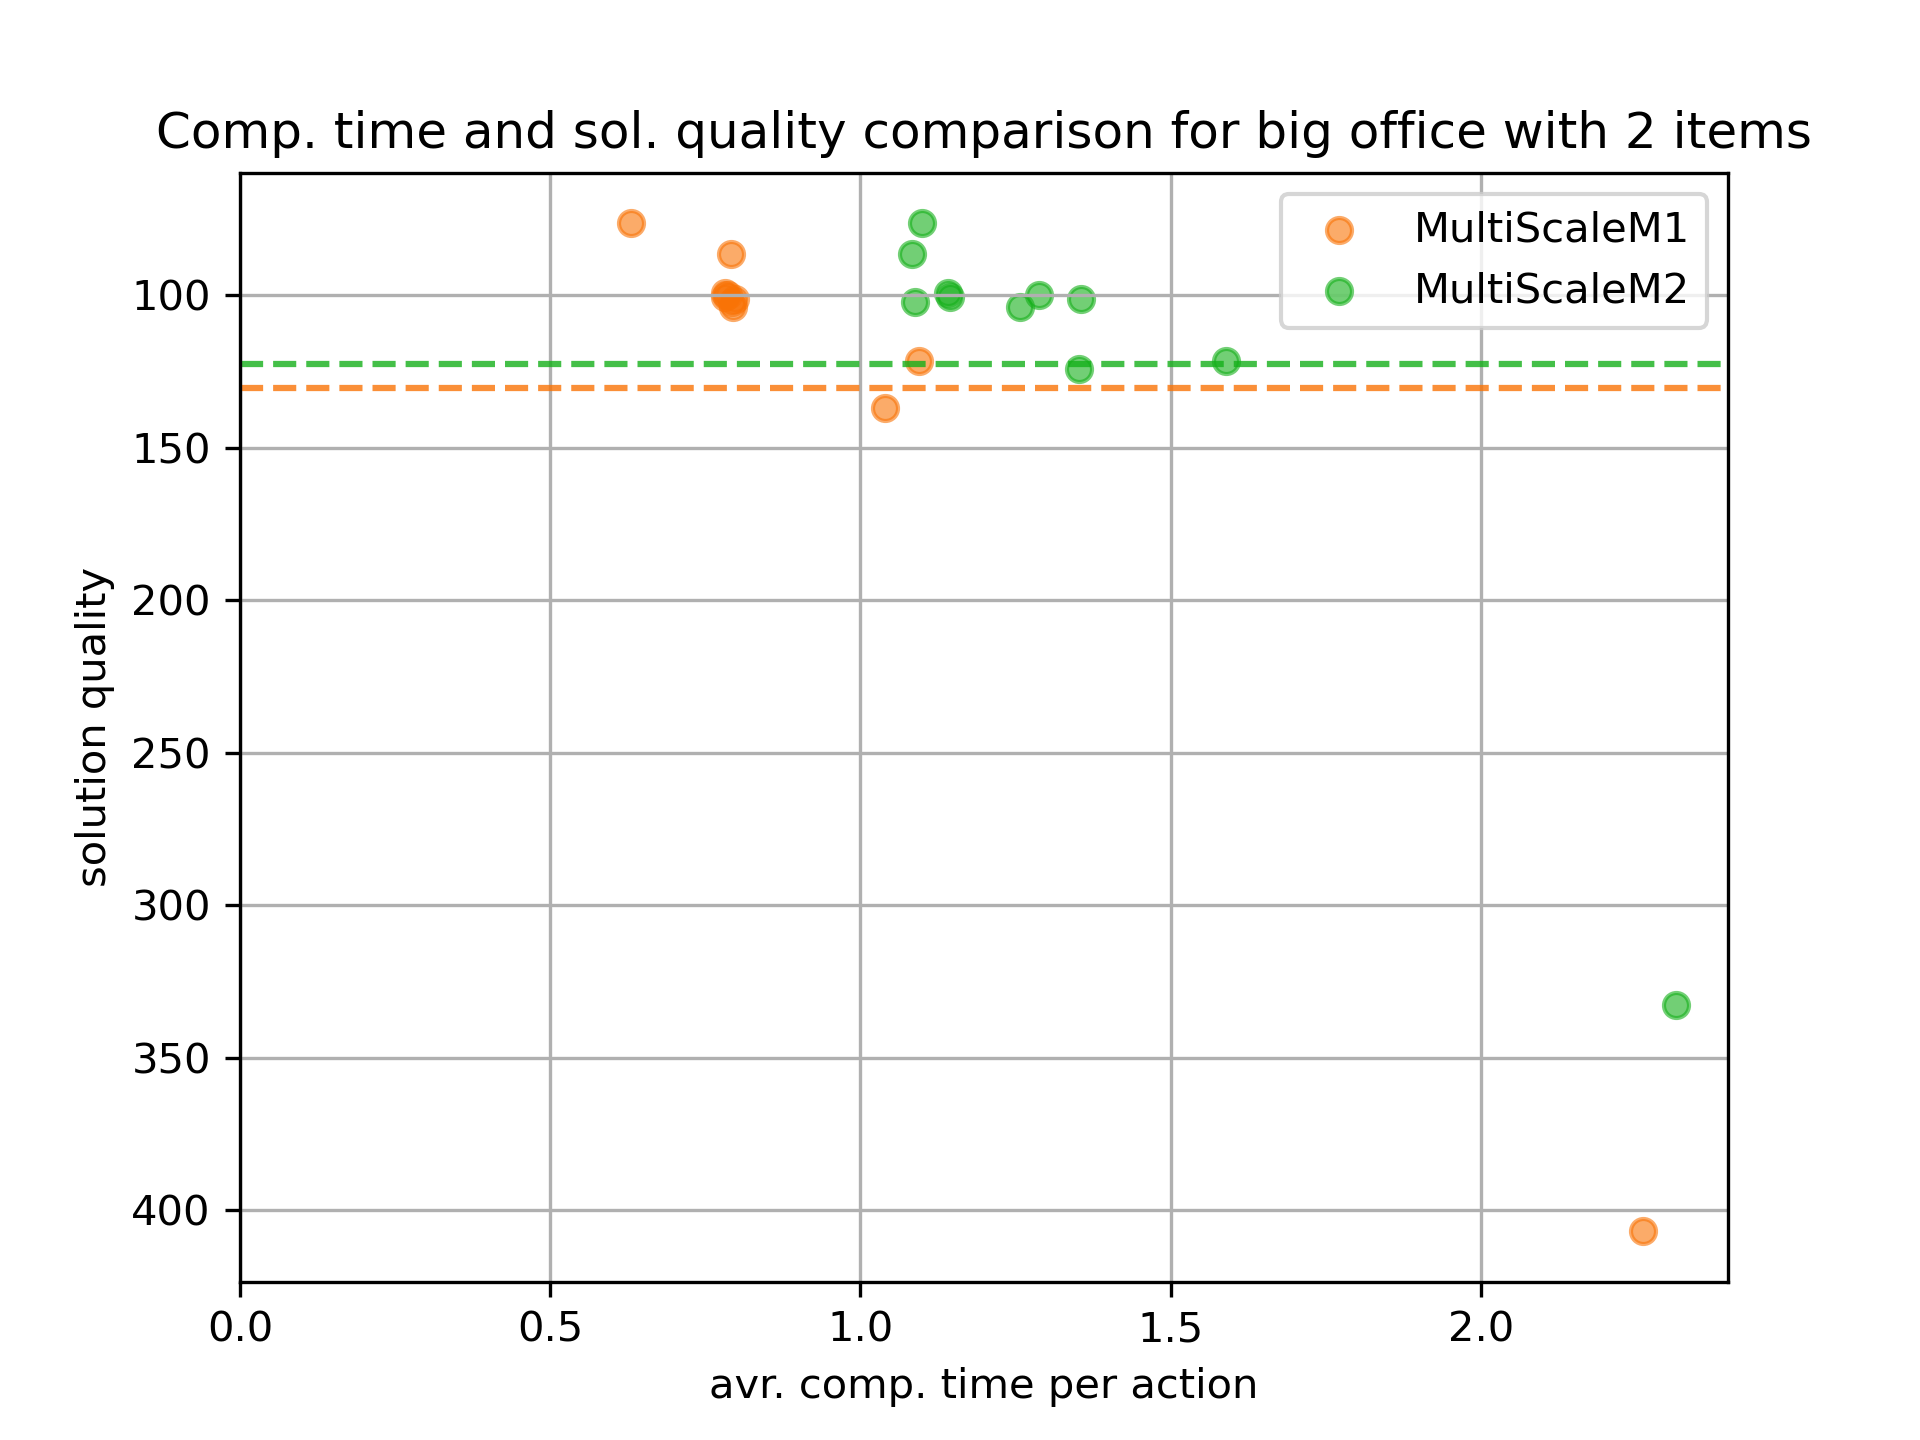
\includegraphics[width=\textwidth]{Report/images/comp_time_vs_sol_quality/envbig_sc03_scatter_comptimes_vs_solqual.png}
        \caption{Two item task in large environment, scenario shown in Figure \ref{subfig:sc03big}}
        \label{subfig:comp_sc03Big}
    \end{subfigure}
    
    \caption{Comparison of the average computation time per action and solution quality for the different agents. The best agents are in the top left corner where both the delivery time (solution quality) and the computation time is short. In (\subref{subfig:comp_sc01}) and (\subref{subfig:comp_sc04}) 100 samples are evaluated,  in (\subref{subfig:comp_sc08}), (\subref{subfig:comp_sc01Big}) and (\subref{subfig:comp_sc03Big}) 30 samples and in (\subref{subfig:comp_sc09}) 10 samples. For the two item scenario in the large environment shown in (\subref{subfig:comp_sc03Big}) only 11 samples are shown as for the other samples the agents did not finish the task before the termination time of the simulation.}
    \label{fig:comptime_vs_solquality}
\end{figure}

In Figure \ref{fig:comptime_vs_solquality} the average computation time per action and the solution time of six different scenarios are plotted for the POMDP agents. Note that the $y$-axis is inverted, such that the runs with the lowest delivery times are on the top of the figure. In Figures \ref{subfig:comp_sc01}-\subref{subfig:comp_sc09} are results for scenarios in the three room environment shown in figure \ref{fig:sc01}. They demonstrate that the Multi-Scale methods yield an order of magnitude speedup without sacrificing solution quality. Further, one can see that from the Multi-Scale agents, Method 01 has on average the lowest and Method 03 the largest computation time which is expected as Method 01 considers the fewest variables on the lower layers and Method 03 the most.
Figure \ref{subfig:comp_sc04} and \ref{subfig:comp_sc08} are both tasks involving two items. The initial belief in (\subref{subfig:comp_sc04}) has three belief peaks while in (\subref{subfig:comp_sc08}) no prior knowledge about the item's location was given, i.e. a uniform belief distribution.\\

In the peaky scenario the solution quality is similar for all agents as only limited reasoning is required to find a good solution. For the broad belief distributions in (\subref{subfig:comp_sc08}) local reasoning of the lower layers becomes more important which explains why Method 02 has shorter delivery times than Method 01.  Method 03 had stability issues and is therefore excluded from the plot. Stability problems mostly occur for broad belief distributions as is explained in Section \ref{sec:M1toM3}. The computation times are longer for the uniform belief scenario as the reachable belief space is larger for the broader initial belief.\\

Figure \ref{subfig:comp_sc09} shows a scenario involving three items. Sarsop was unable to even load the flat POMDP description. The algorithm consumed about 40 GB of RAM before terminating with a segmentation fault error. Method 01 and Method 02 have low computation times while Method 03 is noticeably slower due to its larger state and action space.\\

Plots \ref{subfig:comp_sc01Big}) and \ref{subfig:comp_sc03Big} are scenarios in the large office environment shown in Figure \ref{fig:M1_prob01}. The flat POMDP agent is unable to solve problems this large within reasonable time while the Multi-Scale methods are fast enough for a real-time application. The task in (\subref{subfig:comp_sc01Big}) involves one item. The flat POMDP has an average computation time per action of 300 seconds. Method 01 and Method 02 achieve average computation times below one second and Method 03 below two seconds. For the two item scenario (\subref{subfig:comp_sc03Big}) Method 03 took about 80 seconds for computing an action and is also excluded from the plot. Method 01 and Method 02 still have computation times below two seconds. Note that many samples got removed from the plot as they did not finish the task within the termination time of the simulation. This is a consequence of choosing the termination time too low and that the belief peaks shown in Figure \ref{subfig:sc03big} have a probability of only $0.5$. If the items are not in the expected locations, finding them can take a long time in the large environment. \\


% %%%%%%%%%%%%%%%%%%%%%%%%%%%%%%%%%%%%%%%%%%%%%%%%%%%%%%%%%%%%%%%%%%%%%%%%%%%%%%%%%
% %%%%%%%%%%%%%%%%%%%%%%%%%%%%%%%%%%%%%%%%%%%%%%%%%%%%%%%%%%%%%%%%%%%%%%%%%%%%%%%%%
\begin{figure}[h]
    \centering
    \begin{subfigure}[b]{0.49\textwidth}
        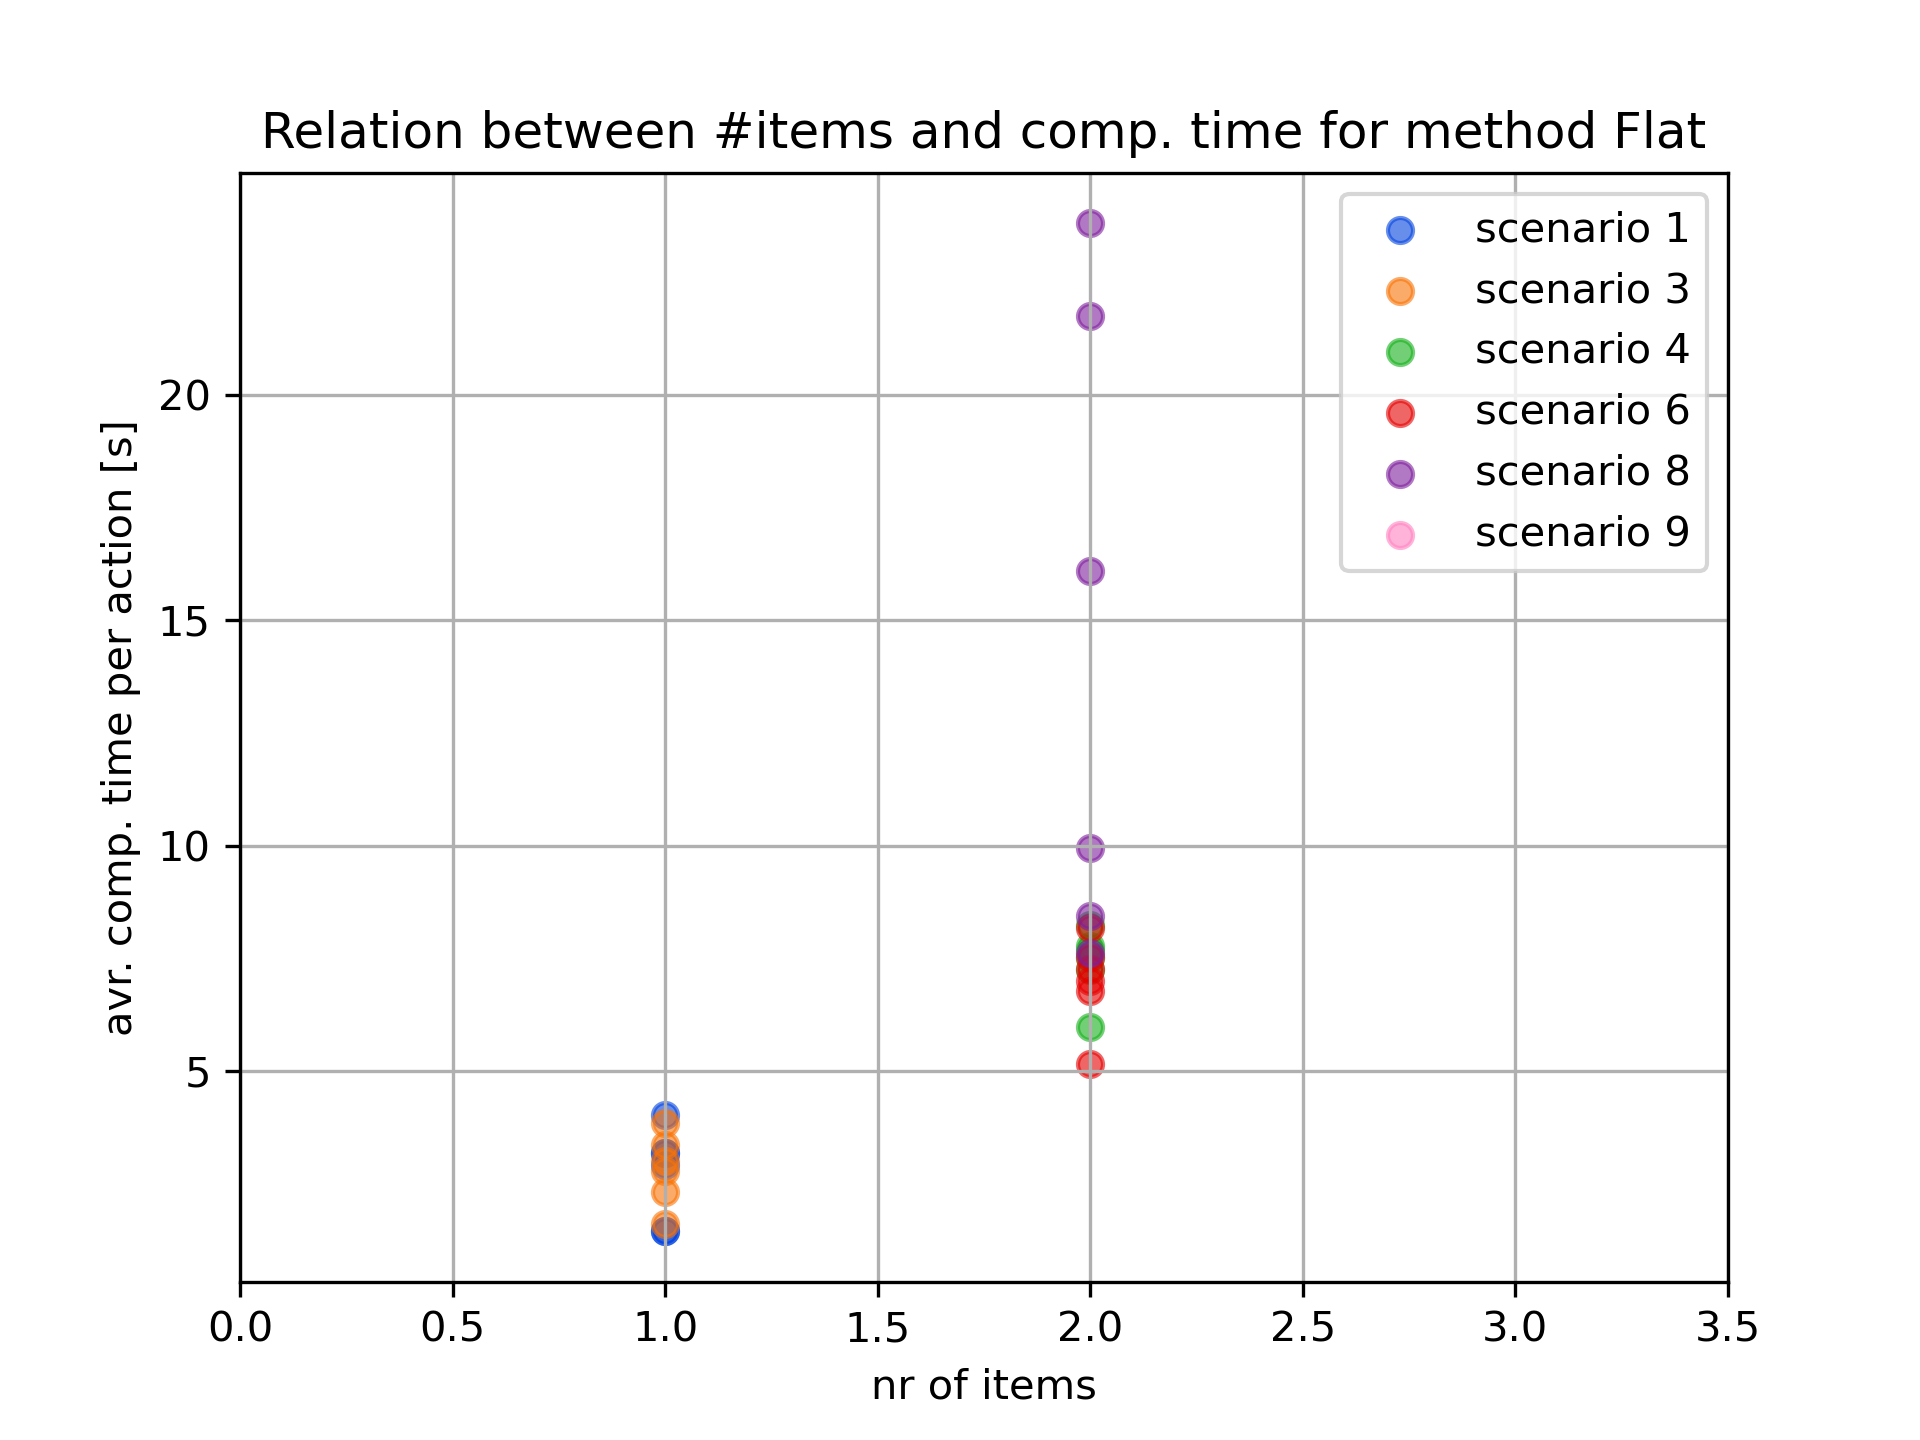
\includegraphics[width=\textwidth]{Report/images/nr_of_items/items_vs_comptime_Flat.png}
        \caption{Flat POMDP agent}
        \label{subfig:nr_of_items_Flat}
    \end{subfigure}
    \begin{subfigure}[b]{0.49\textwidth}
         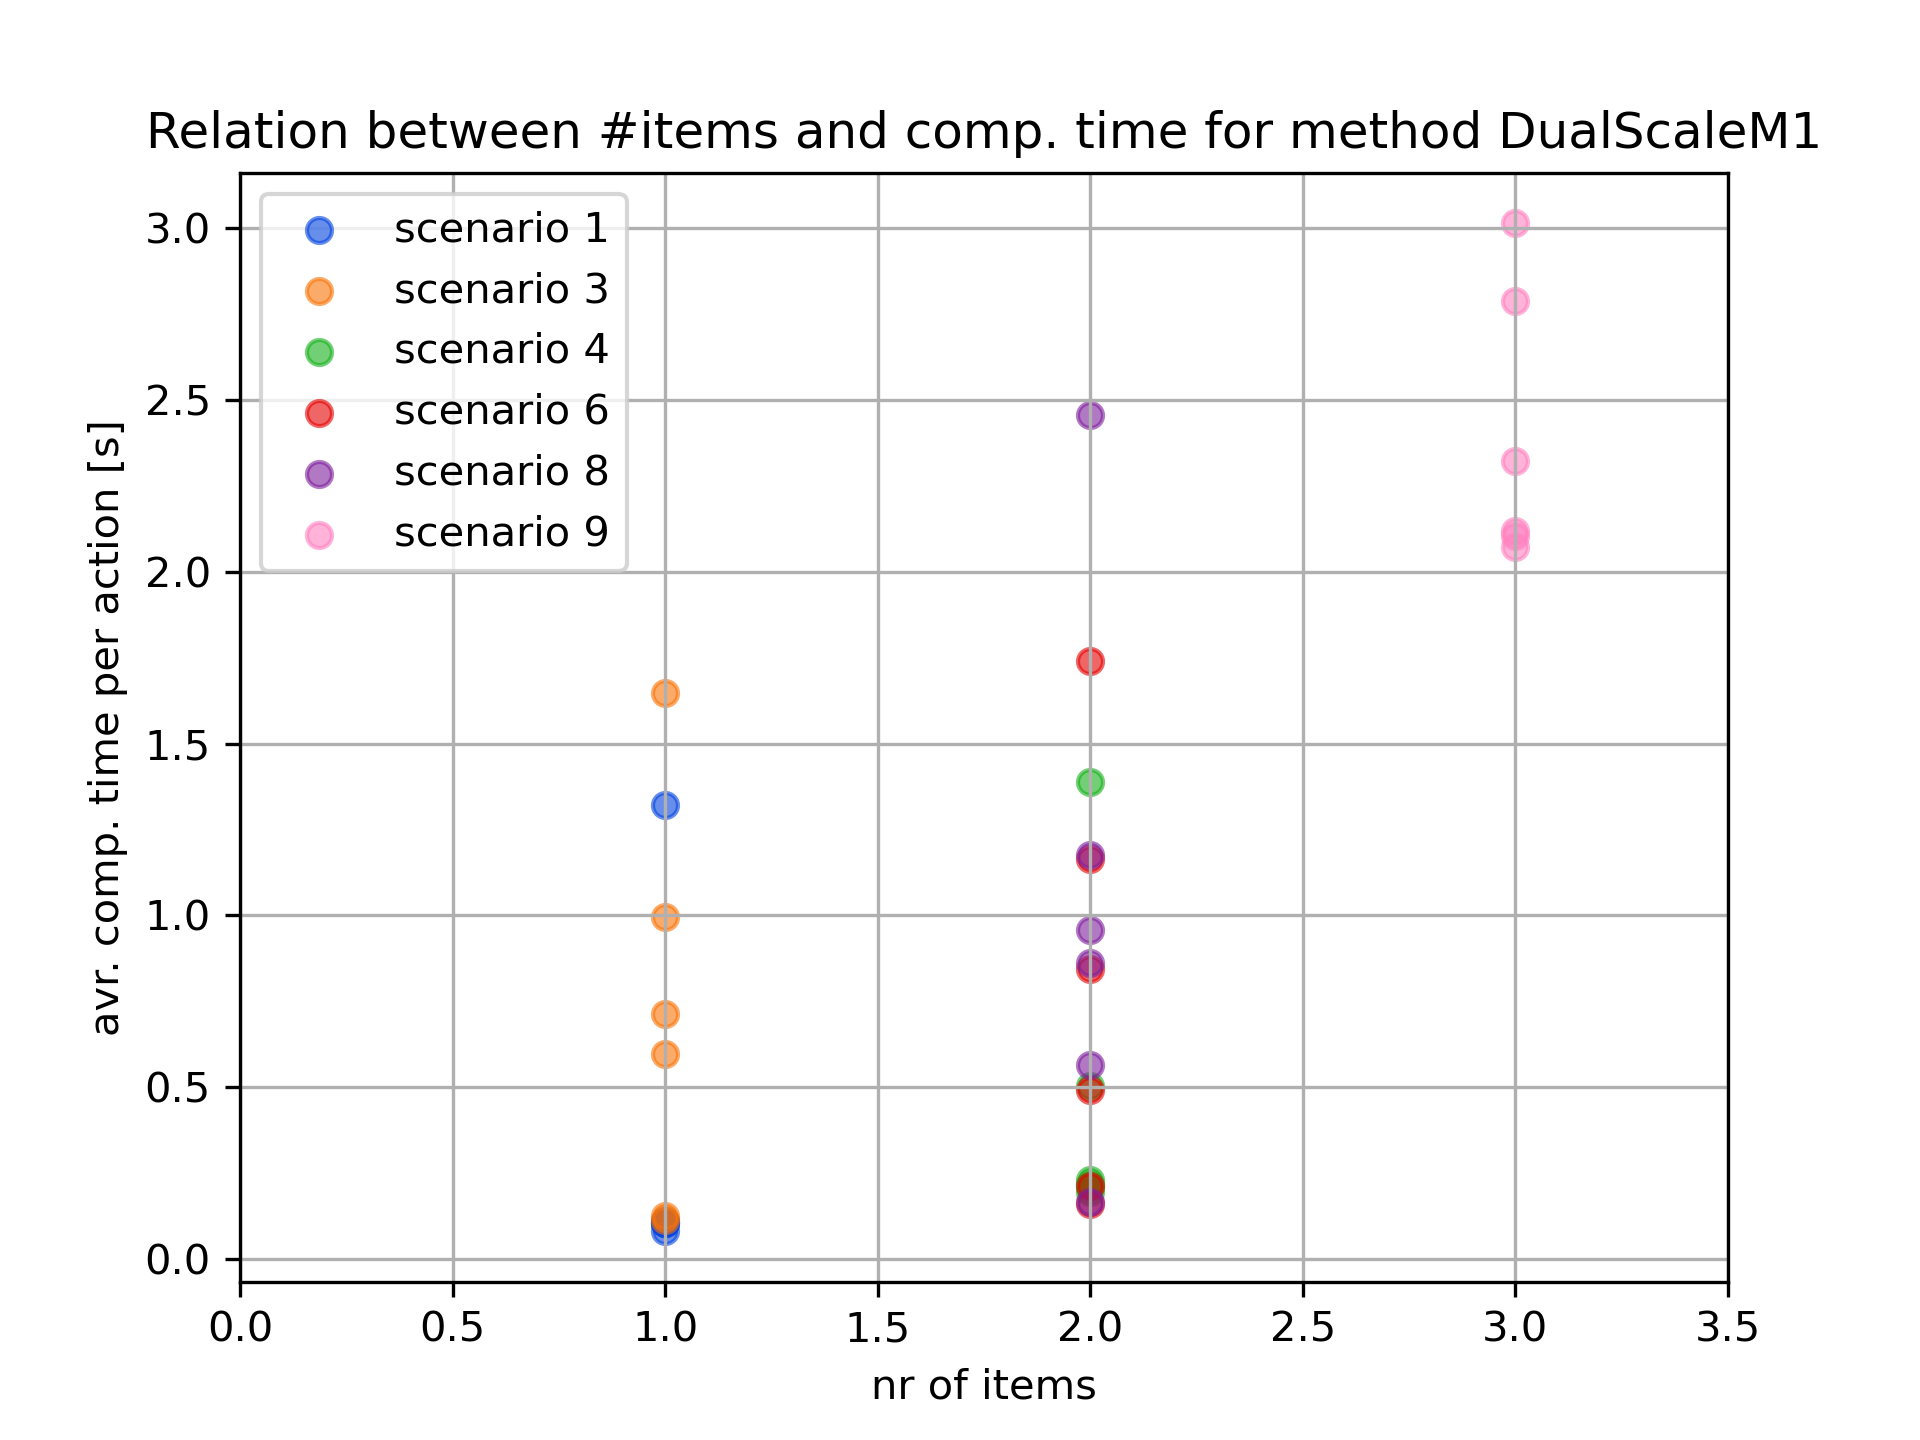
\includegraphics[width=\textwidth]{Report/images/nr_of_items/items_vs_comptime_DualScaleM1.png}
        \caption{Multi-Scale Method 01 agent}
        \label{subfig:nr_of_items_D1}
    \end{subfigure}
    \hfill
    \begin{subfigure}[b]{0.49\textwidth}
        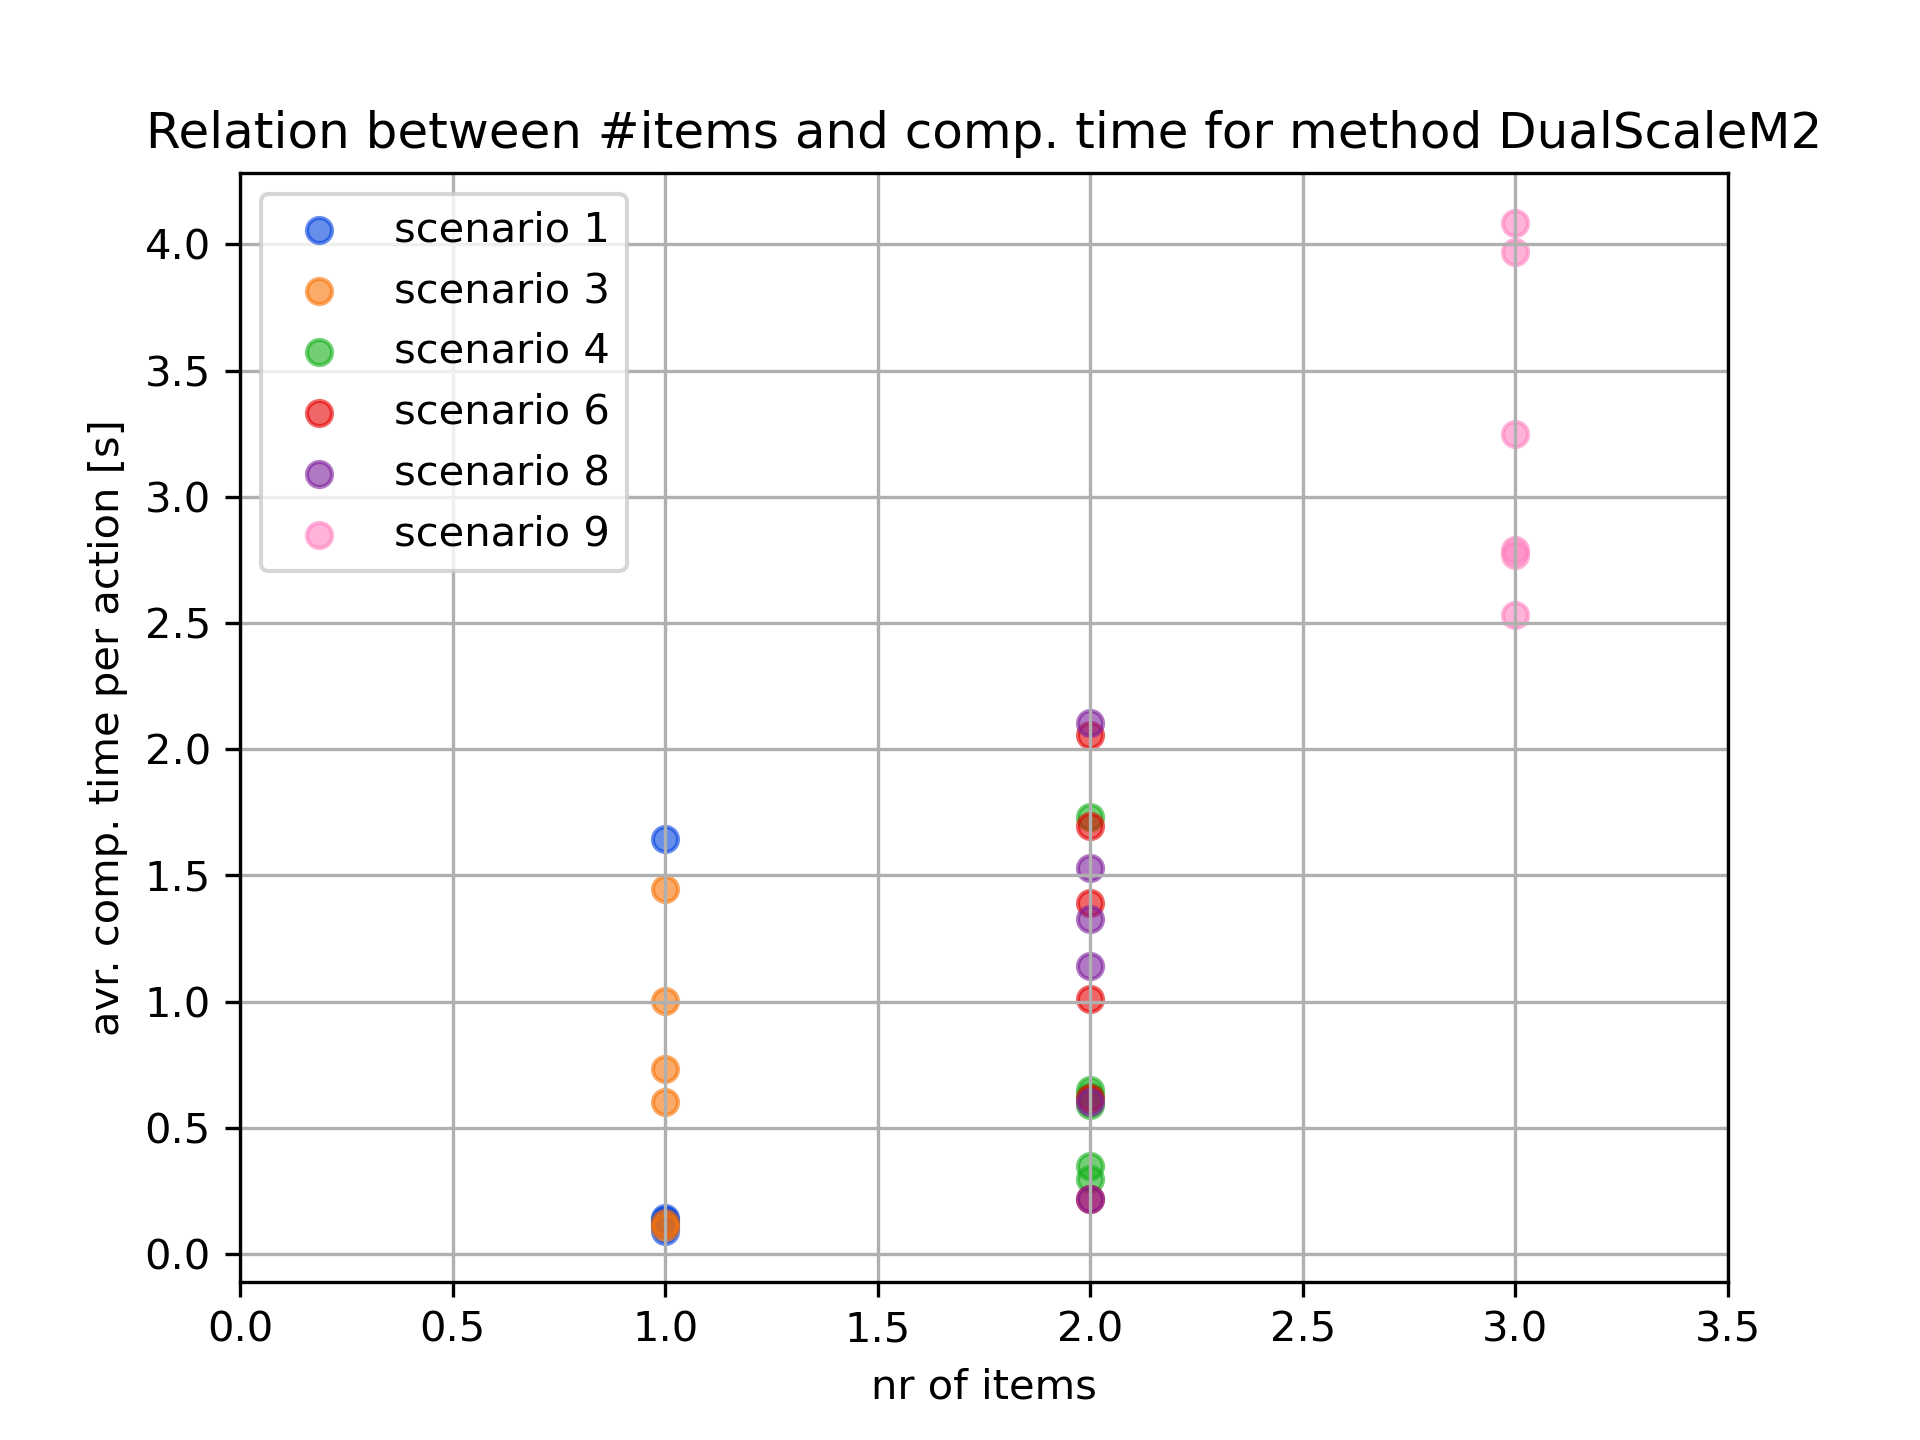
\includegraphics[width=\textwidth]{Report/images/nr_of_items/items_vs_comptime_DualScaleM2.png}
        \caption{Multi-Scale Method 02 agent}
        \label{subfig:nr_of_items_D2}
    \end{subfigure}
    \hfill
    \begin{subfigure}[b]{0.49\textwidth}
         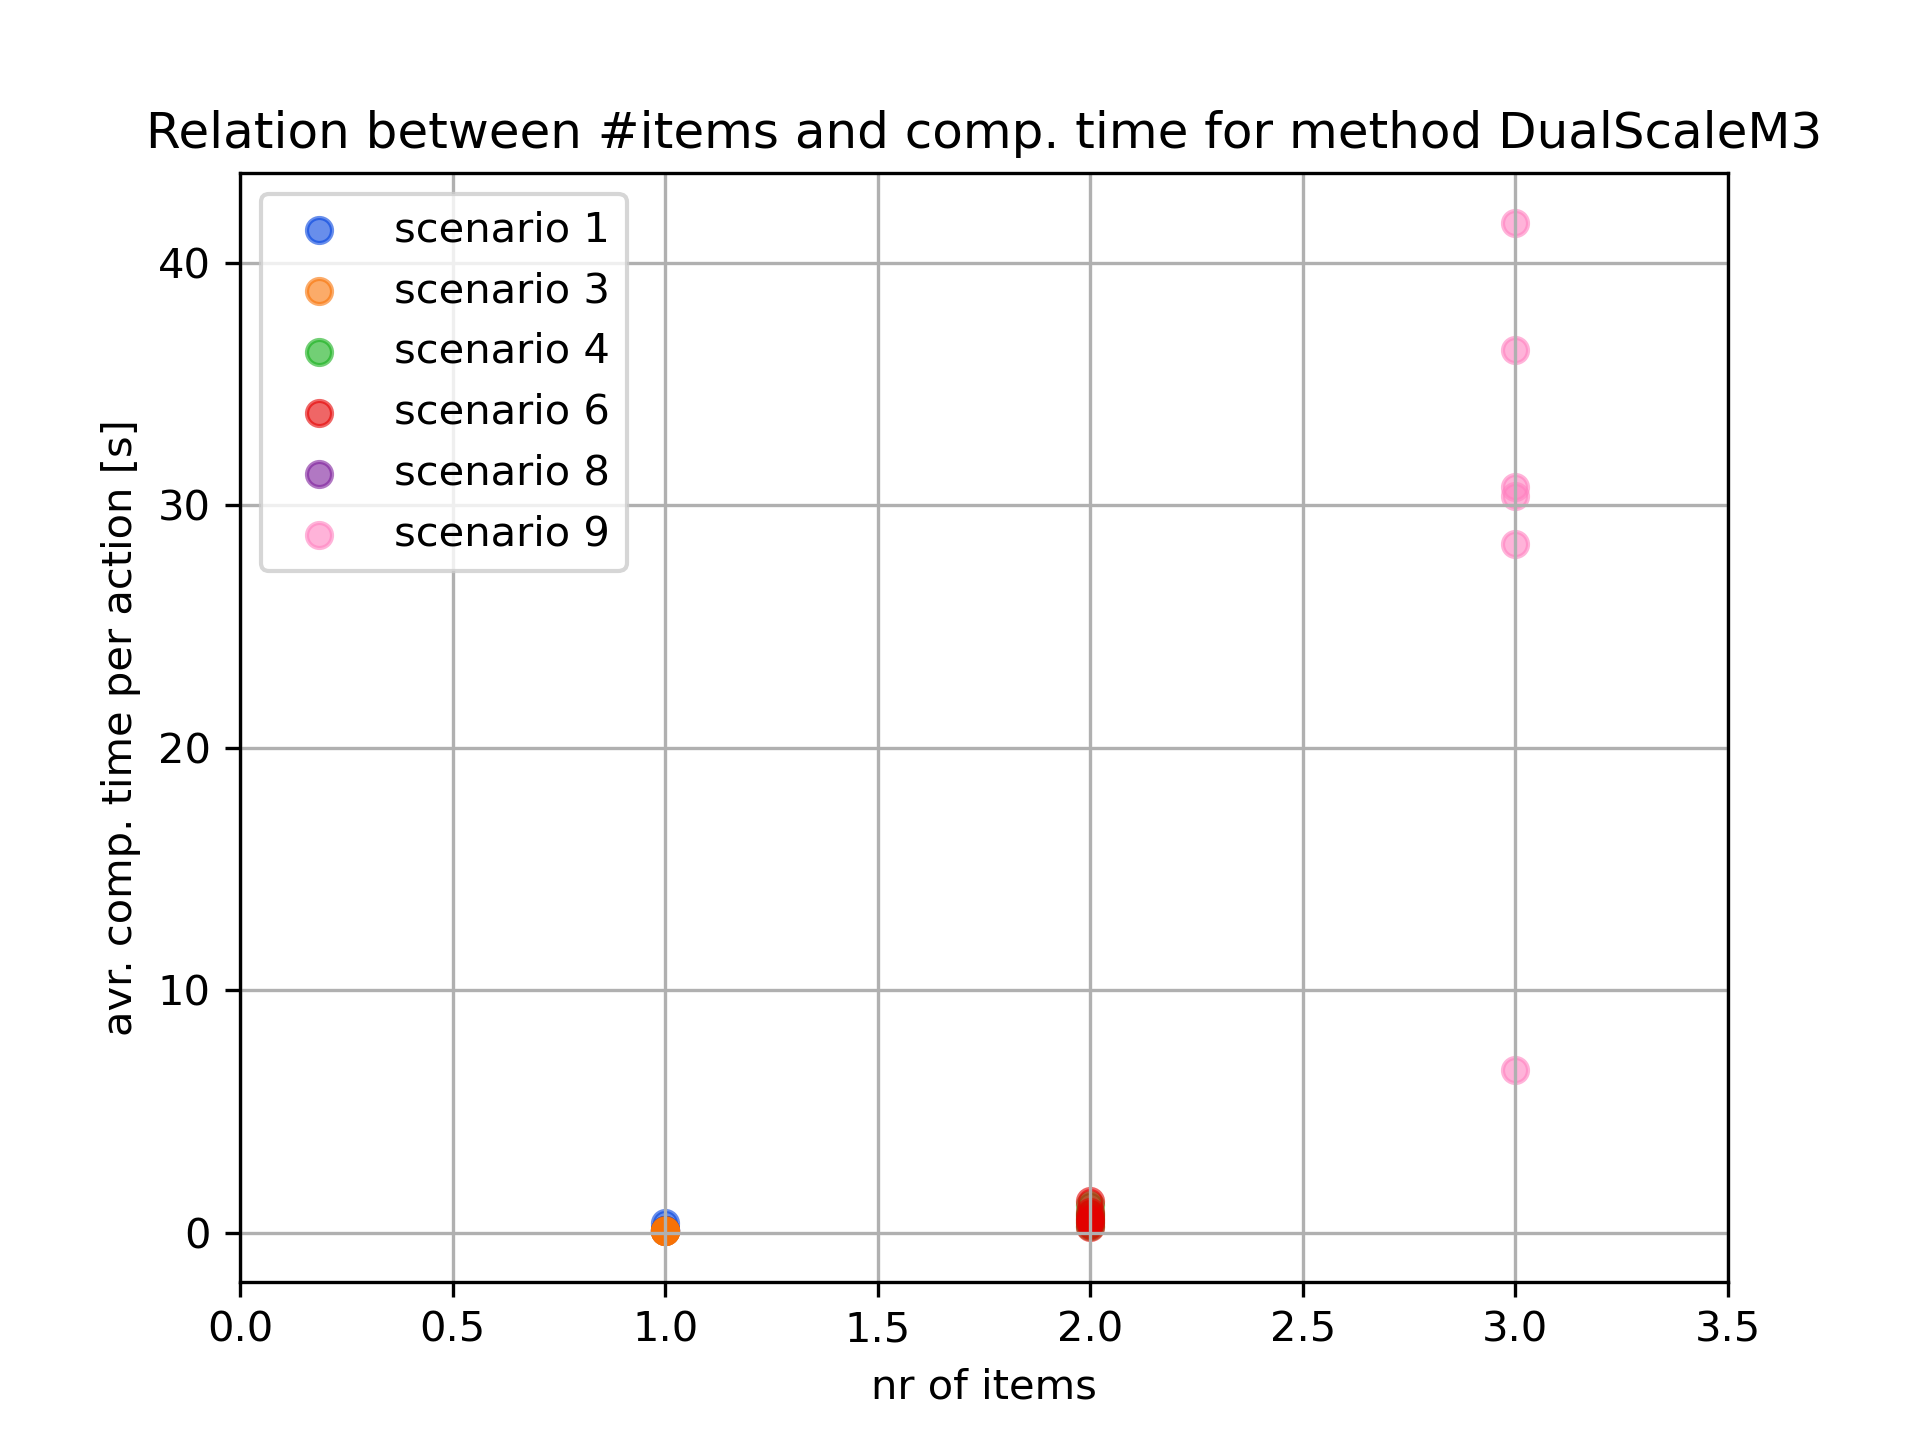
\includegraphics[width=\textwidth]{Report/images/nr_of_items/items_vs_comptime_DualScaleM3.png}
        \caption{Multi-Scale Method 03 agent}
        \label{subfig:nr_of_items_D3}
    \end{subfigure}
     \caption{Influence of the number of items in the task on the average computation time per action. All six scenarios take place in the small office environment but have different initial belief distributions. Scenario 3 has a broader belief than Scenario~1. Scenario 8 has a uniform belief distribution and scenario 6 has a broader initial belief than Scenario 4.}
    \label{fig:nr_of_items}
\end{figure}
In Figure \ref{fig:nr_of_items} the influence of the number of items in the task on computation time is shown for the four POMDP methods. The scenarios plotted have varying ‘‘peakiness’’ of the initial belief distribution. One can see that the number of items considered has a greater effect on computation time than the specific belief distribution. The state-action space increases exponentially with the number of items and so does the computation time. The average computation time of Method 01 grows the least per extra item. This coincides with the fact that for Method 01 only the top layer considers all items while the lower layers consider at most one item. For Method 03 the computation time for three items is already a magnitude higher than for two items. As Method 03 considers more nodes than Method 01 and Method 02, the exponential growth can already be observed for three items. For the flat POMDP agent a three item scenario could not be computed for reasons stated above.
%%%%%%%%%%%%%%%%%%%%%%%%%%%%%%%%%%%%%%%%%%%%%%%%%%%%%%%%%%%%%%%%%%%
%%%%%%%%%%%%%%%%%%%%%%%%%%%%%%%%%%%%%%%%%%%%%%%%%%%%%%%%%%%%%%%%%%%

\section{Corner Cases}\label{sec:cornercases}
In this section the reasoning abilities of the three Multi-Scale methods are compared on two scenarios highlighting the limitations of the individual agents. The first problem shown in Figure \ref{fig:M1_prob01} demonstrates that Method 02 and Method 03 have better lower layer reasoning than Method 01. In (\subref{subfig:problem1_M1}) and (\subref{subfig:problem1_M2}) a snapshot of the Method 01 and Method 02 agents is shown. In the task, the item is located right at the corner of one of multiple belief peaks, such that it was not spotted by the navigation action. For Method 01 the top layer decided to go to node $n_0^{l0}$ as the majority of the belief peak was observed. The coarse discretisation of layer 0 does not reflect that some part of the belief peak is right in front of the agent. Similarly, the search in the bottom right-most room was more thorough than in the one left of it. As the belief in $n_3^{l0}$ decreased under a certain threshold, layer 0 chose to go the another node. The lower layers of Method 01 execute the action of the layer above in as little time as possible and can not correct for the top layer's inaccuracy.
Method 02 has better lower layer reasoning than Method 01 and finds the item right away. As for Method 01, the top layer decides to go to $n_0^{l0}$. The lower layers in Method 02 have access to the value function of the layer above and can choose to first explore the current states before completing the higher layer action. Layer 1 chose a \texttt{look\_around} action and observes the item, leading to a better solution than the one of Method 01. \\

\begin{figure}[b]
    \centering
    \begin{subfigure}[b]{0.49\textwidth}
        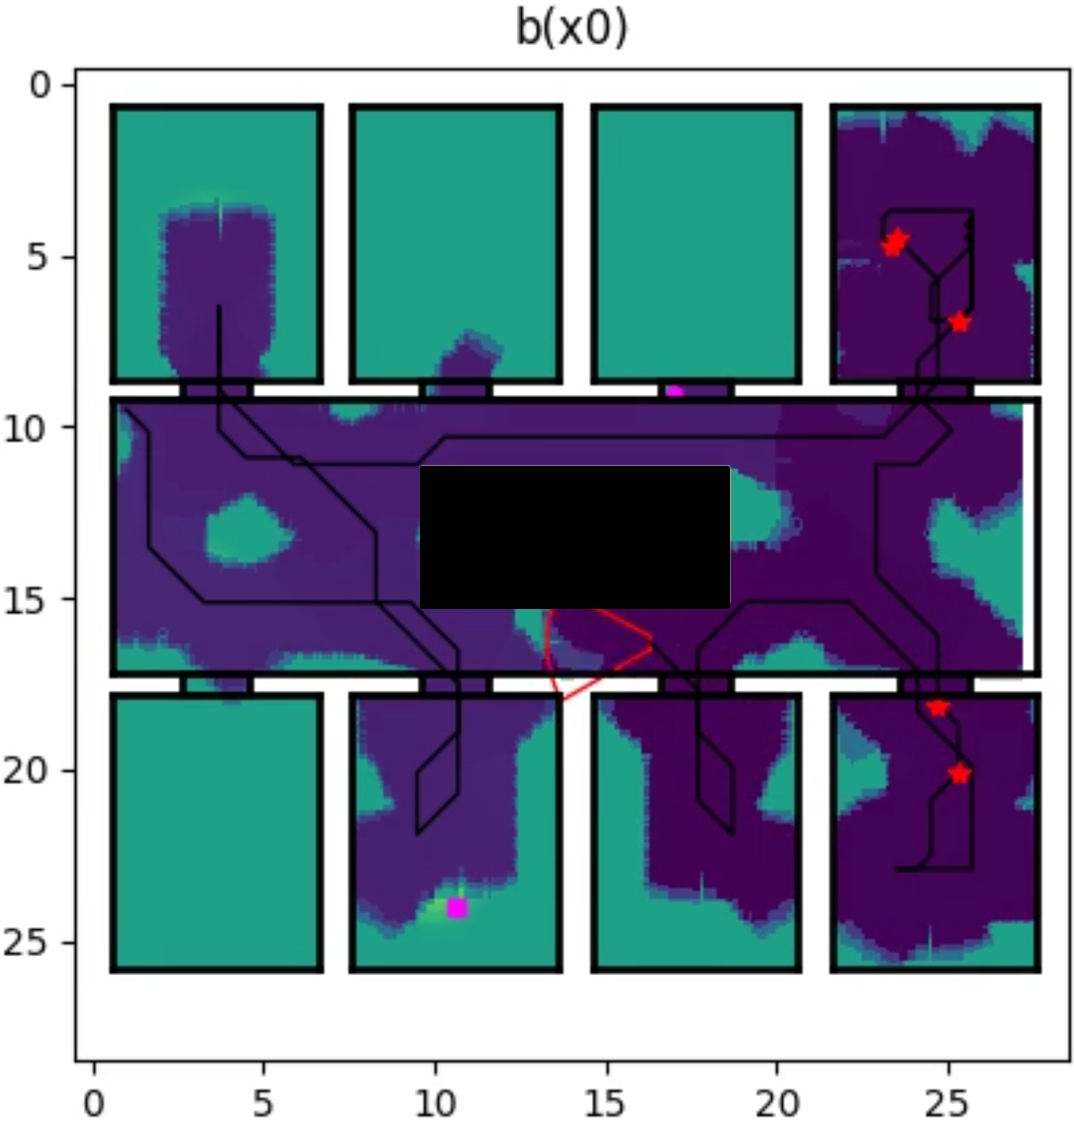
\includegraphics[width=\textwidth]{Report/images/experiments/M1_envbig_problem1_blackbox.png}
        \caption{Method 01}
        \label{subfig:problem1_M1}
    \end{subfigure}
    \begin{subfigure}[b]{0.49\textwidth}
         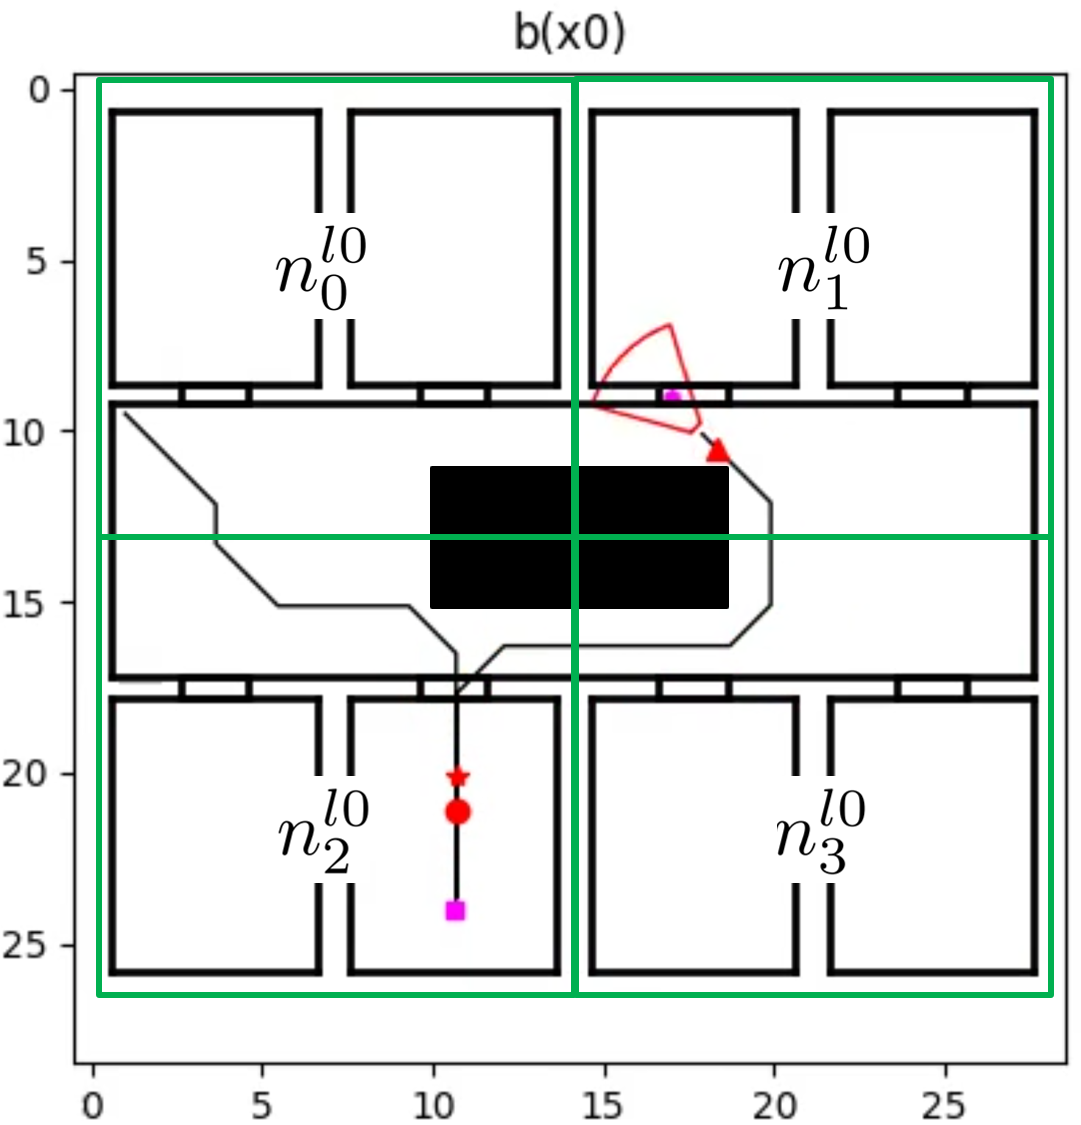
\includegraphics[width=\textwidth]{Report/images/experiments/M2_envbig_problem1_nodes.png}
        \caption{Method 02}
        \label{subfig:problem1_M2}
    \end{subfigure}
    \caption{Demonstration of inconsistent search behaviour of Method 01 shown in (a) compared to Method 02 in (b). The Method 01 agent missed the item right at the corner of the belief peak and continued its search in other rooms. Some rooms are searched much more thoroughly than others. Method 02 spends more time exploring the first room and finds the item right away. The black lines show the previous path of the agent, the red stars are \texttt{look\_around} action, the red circle is a pickup action and the red triangle is the \texttt{release} action.}
    \label{fig:M1_prob01}
\end{figure}

The second example shown in Figure \ref{subfig:problem2_M1} explores a scenario where both Method 01 and Method 02 choose a suboptimal path to get to the target location due to coarse resolution of the top layer. Method 03 shown in (\subref{subfig:problem2_M3}) can correct for the inaccuracies and chooses the shorter path. Consider the layer 0 discretisation for the large office environment in (\subref{subfig:problem2_M1}). The item shown as a pink square lies within node $n_0^{l0}$ and its goal location in $n_3^{l0}$. There is no direct connection between $n_0^{l0}$ and $n_3^{l0}$ so the layer 0 POMDP has to navigate either over $n_1^{l0}$ or over $n_2^{l0}$ to get to $n_3^{l0}$. Due to the symmetry of the node layout, layer 0 cannot reason over which path is better suited and chooses the longer path over $n_2^{l0}$. The lower layer POMDPs of both Method 01 and Method 02 execute the proposed action of the above layer. In Method 03, the lower layers have complete freedom and are only guided through the value function of the layer above. The lower layers recognize that the agent is closer to $n_1^{l0}$ than to $n_2^{l0}$ and takes the shorter way.

%%%%%%%%%%%%%%%%%%%%%%%%%%%%%%%%%%%%%%%%%%%%%%%%%%%%%%%%%%%%%%
%%%%%%%%%%%%%%%%%%%%%%%%%%%%%%%%%%%%%%%%%%%%%%%%%%%%%%%%%%%%
\begin{figure}
    \centering
    \begin{subfigure}[b]{0.49\textwidth}
        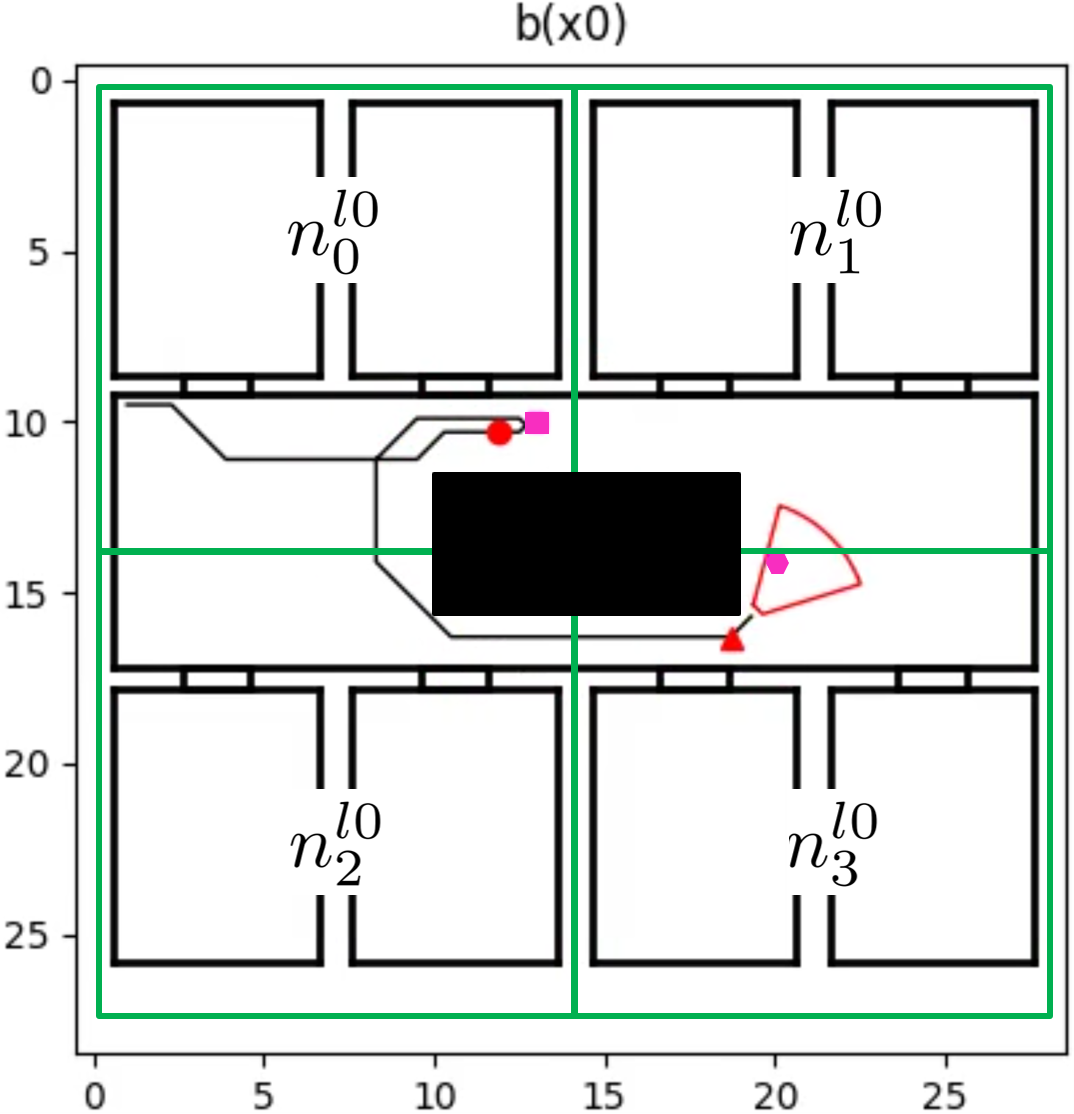
\includegraphics[width=\textwidth]{Report/images/experiments/M1_envbig_problem2_nodes.png}
        \caption{Method 01}
        \label{subfig:problem2_M1}
    \end{subfigure}
    \begin{subfigure}[b]{0.49\textwidth}
         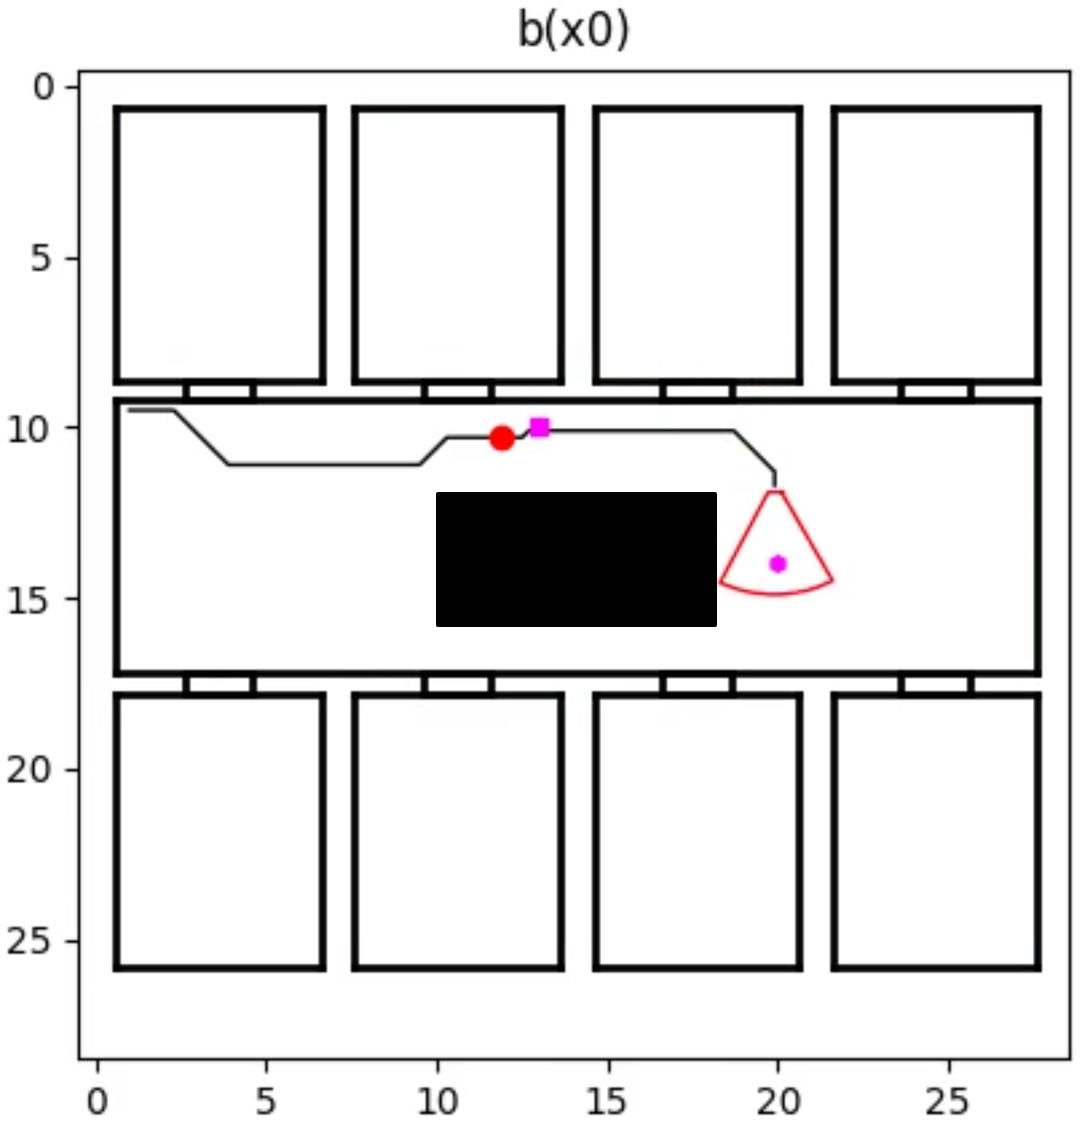
\includegraphics[width=\textwidth]{Report/images/experiments/M3_envbig_problem2_blackbox.png}
        \caption{Method 03}
        \label{subfig:problem2_M3}
    \end{subfigure}
    \caption{Demonstration of limited lower layer reasoning for method 01 shown in (a) compared to the better reasoning of method 03 in (b). Because of the coarse resolution, layer 0 is not able to correctly reason if the path over $n_1^{l1}$ or over $n_2^{l1}$ is faster for reaching the goal location. Method 03 is not restricted to follow the higher layer actions and correctly reasons that the path over $n_1^{l0}$ is faster.}
    \label{fig:M1_prob02}
\end{figure}
%%%%%%%%%%%%%%%%%%%%%%%%%%%%%%%%%%%%%%%%%%%%%%%
\begin{figure}
    \centering
    %
    \begin{subfigure}[b]{0.49\textwidth}
        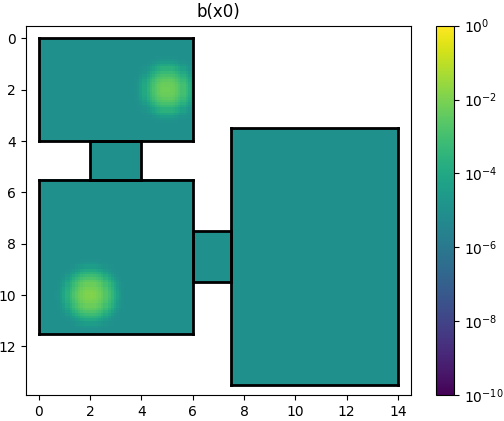
\includegraphics[width=\textwidth]{Report/images/scenarios/envsmall_sc01.png}
        \caption{Small office, Scenario 01}
        \label{subfig:sc01}
    \end{subfigure}
    %
    \hfill
     \begin{subfigure}[b]{0.49\textwidth}
        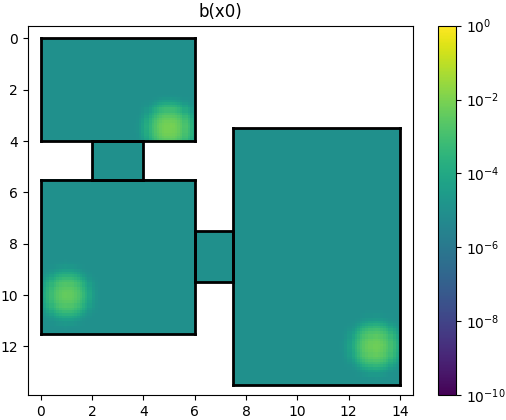
\includegraphics[width=\textwidth]{Report/images/scenarios/envsmall_sc03.png}
        \caption{Small office, Scenario 03}
        \label{subfig:sc03}
    \end{subfigure}
    %
     \begin{subfigure}[b]{\textwidth}
        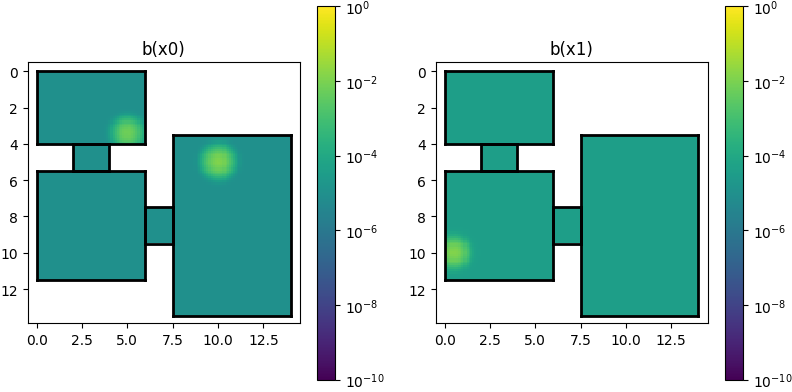
\includegraphics[width=\textwidth]{Report/images/scenarios/envsmall_sc04.png}
        \caption{Small office, Scenario 04}
        \label{subfig:sc04}
    \end{subfigure}
    %
     \begin{subfigure}[b]{\textwidth}
        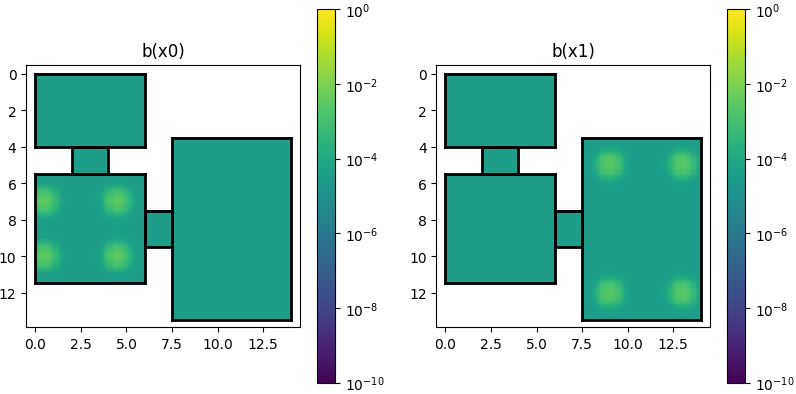
\includegraphics[width=\textwidth]{Report/images/scenarios/envsmall_sc06.png}
        \caption{Small office, Scenario 06}
        \label{subfig:sc06}
    \end{subfigure}
    %
    \caption{Initial belief grid of the tested scenarios.}
    \label{fig:scenarios}
\end{figure}
%
\begin{figure}\ContinuedFloat
    \centering
    %
    \begin{subfigure}[b]{\textwidth}
        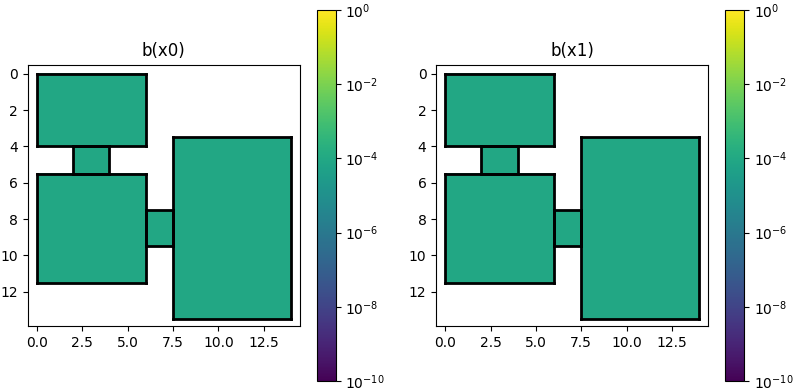
\includegraphics[width=\textwidth]{Report/images/scenarios/envsmall_sc08.png}
        \caption{Small office, Scenario 08}
        \label{subfig:sc08}
    \end{subfigure}
    %
     \begin{subfigure}[b]{\textwidth}
        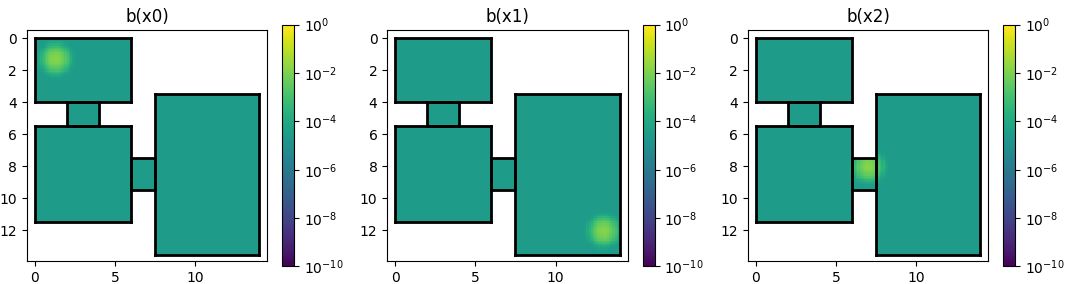
\includegraphics[width=\textwidth]{Report/images/scenarios/envsmall_sc09.png}
        \caption{Small office Scenario 09}
        \label{subfig:sc09}
    \end{subfigure}
    %
    \centering
    \begin{subfigure}[c]{0.5\textwidth}
        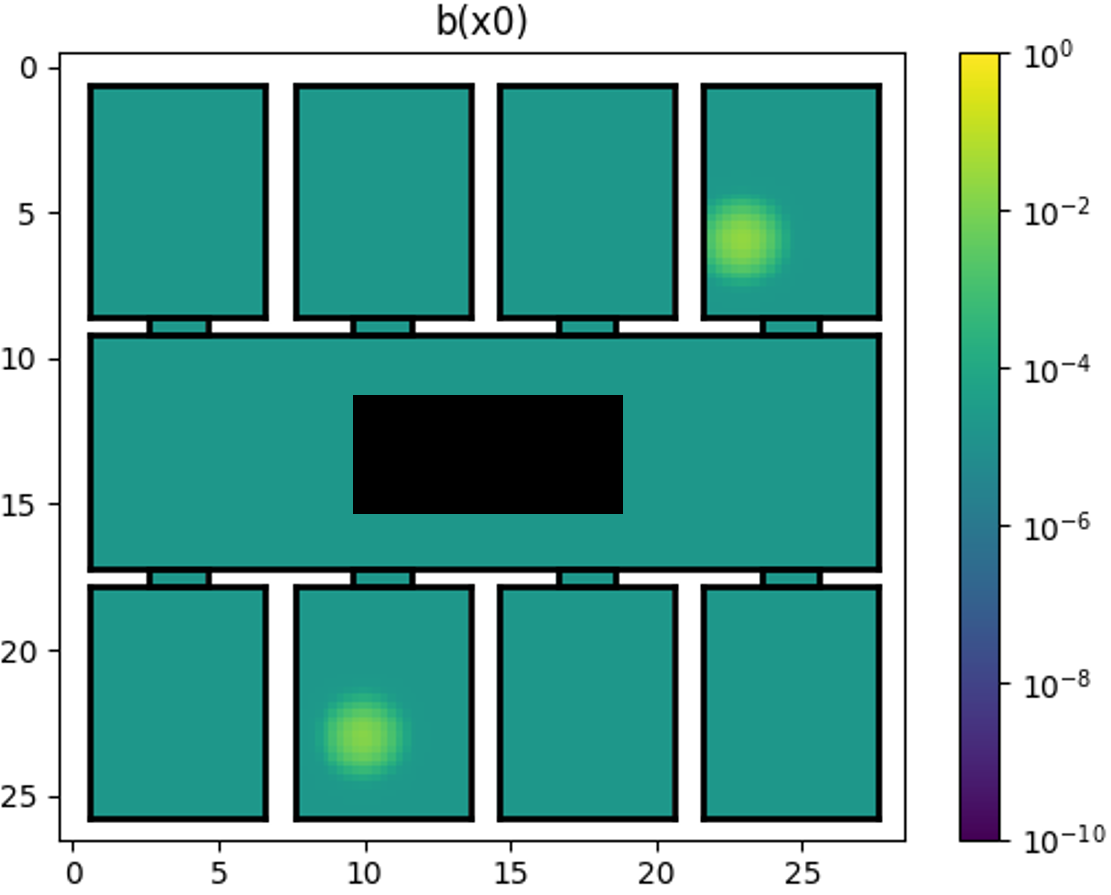
\includegraphics[width=\textwidth]{Report/images/scenarios/envbig_sc01_a.png}
        \caption{Big office, Scenario 01}
        \label{subfig:sc01big}
    \end{subfigure}
    %
     \begin{subfigure}[t]{\textwidth}
        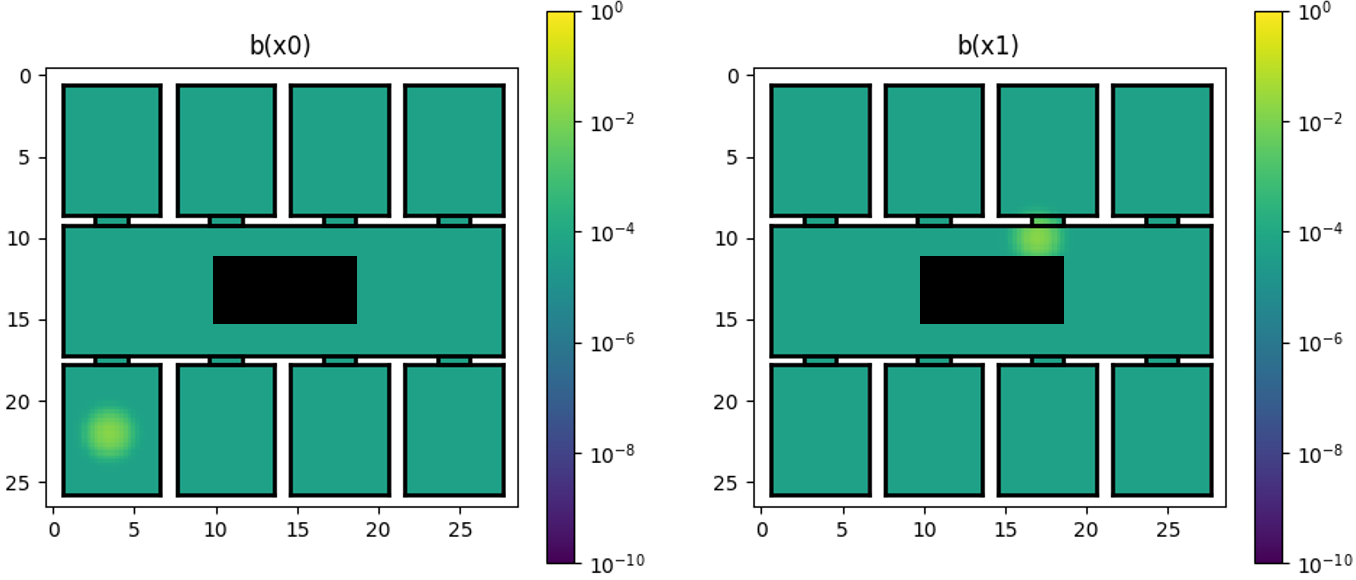
\includegraphics[width=\textwidth]{Report/images/scenarios/envbig_sc03_a.png}
        \caption{Big office, Scenario 03}
        \label{subfig:sc03big}
    \end{subfigure}
    \repeatcaption{fig:scenarios}{Initial belief grid of the tested scenarios.}
    %\label{fig:scenarios}
\end{figure}
